%! TEX encoding = utf8
\chapter{Regulacja z skokowym zakłóceniem sinusoidalnym}

Szum pomiarowy generowano poleceniem wgn() i dodawano go do ustawionej wartości zakłócenia

\section{Szum nałożony na zakłócenie skokowe}

\begin{figure}[H]
\centering
% This file was created by matlab2tikz.
%
%The latest updates can be retrieved from
%  http://www.mathworks.com/matlabcentral/fileexchange/22022-matlab2tikz-matlab2tikz
%where you can also make suggestions and rate matlab2tikz.
%
\definecolor{mycolor1}{rgb}{0.00000,0.44700,0.74100}%
%
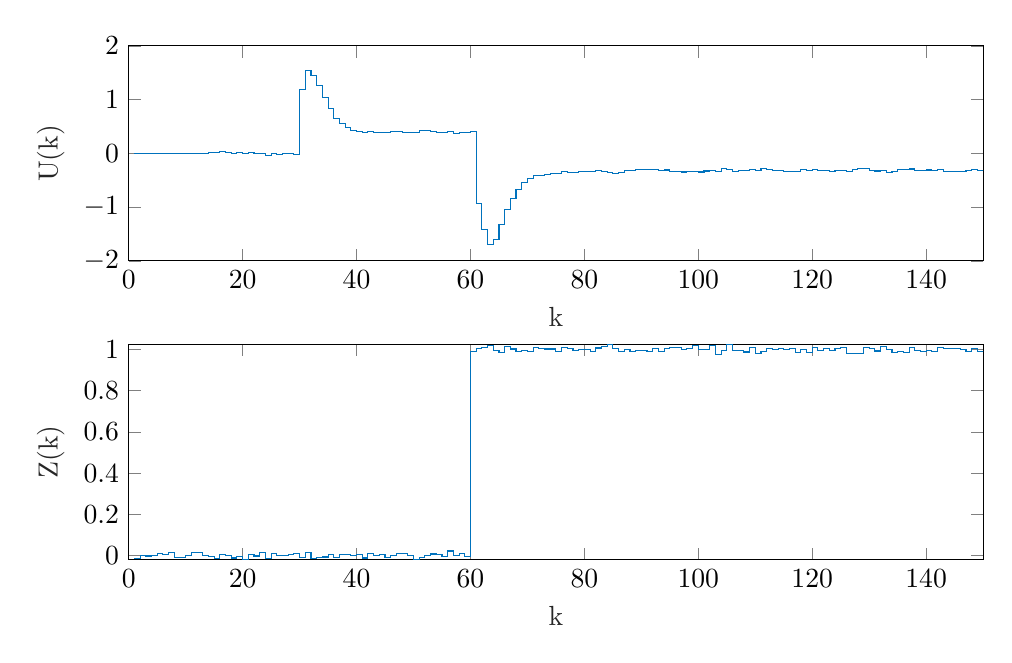
\begin{tikzpicture}

\begin{axis}[%
width=4.272in,
height=1.075in,
at={(0.717in,1.839in)},
scale only axis,
xmin=0,
xmax=150,
xlabel style={font=\color{white!15!black}},
xlabel={k},
ymin=-2,
ymax=2,
ylabel style={font=\color{white!15!black}},
ylabel={U(k)},
axis background/.style={fill=white}
]
\addplot[const plot, color=mycolor1, forget plot] table[row sep=crcr] {%
1	0\\
2	0\\
3	0\\
4	0\\
5	0\\
6	0\\
7	0\\
8	0\\
9	0\\
10	0\\
11	0\\
12	0.000434587682167119\\
13	0.000243916940038817\\
14	0.0148660254779791\\
15	0.0227060712444275\\
16	0.0369278289165441\\
17	0.00808439480099233\\
18	0.00335351157592429\\
19	0.0101185113717708\\
20	0.00193286246509215\\
21	0.0209268804832885\\
22	-0.00613364717555564\\
23	-0.00572037393958827\\
24	-0.0353851146579039\\
25	-0.00225970448500858\\
26	-0.0231040343288302\\
27	-0.0107831986147378\\
28	-0.00978575951776835\\
29	-0.0146939963465967\\
30	1.18382673086061\\
31	1.54451008043006\\
32	1.45111273299934\\
33	1.26433272959979\\
34	1.03058592102796\\
35	0.828400315680257\\
36	0.653515734063443\\
37	0.561219052519699\\
38	0.475207620449167\\
39	0.430620238522634\\
40	0.406739146591162\\
41	0.390277638993814\\
42	0.408720936804318\\
43	0.385985687119288\\
44	0.394208863828704\\
45	0.384541142444709\\
46	0.407898987098295\\
47	0.40199698129465\\
48	0.392368027238047\\
49	0.384000594897505\\
50	0.394862045955653\\
51	0.424205975647106\\
52	0.427375185054801\\
53	0.412139824077039\\
54	0.393710183592335\\
55	0.387412663490683\\
56	0.399741477509157\\
57	0.368000346350359\\
58	0.38959394145227\\
59	0.382276269341309\\
60	0.40425880600975\\
61	-0.93662012576268\\
62	-1.41874098350105\\
63	-1.69942920985893\\
64	-1.60227974852856\\
65	-1.32576279787853\\
66	-1.03948608815925\\
67	-0.847936190459632\\
68	-0.672939397481384\\
69	-0.542015874811265\\
70	-0.463104603015313\\
71	-0.407704409676296\\
72	-0.405125706900011\\
73	-0.389840198710596\\
74	-0.378822379465069\\
75	-0.36837116325726\\
76	-0.345601422830382\\
77	-0.359572769519619\\
78	-0.352238823084512\\
79	-0.343869127180721\\
80	-0.338174786375953\\
81	-0.33463588419947\\
82	-0.322387254471842\\
83	-0.340027290482996\\
84	-0.353526091383658\\
85	-0.375668264346881\\
86	-0.354850116483786\\
87	-0.326820011745535\\
88	-0.322847993895688\\
89	-0.302340092877798\\
90	-0.304406086231478\\
91	-0.304102886471742\\
92	-0.305093608237757\\
93	-0.323739440407527\\
94	-0.311044130360401\\
95	-0.333433211840762\\
96	-0.339528038477274\\
97	-0.347952726502402\\
98	-0.334200288409619\\
99	-0.335543132543132\\
100	-0.347884142734273\\
101	-0.328805795829051\\
102	-0.31946396740704\\
103	-0.337540332787026\\
104	-0.285940633259678\\
105	-0.299877223645811\\
106	-0.336756666178557\\
107	-0.318519178062558\\
108	-0.316552033384519\\
109	-0.298917030961772\\
110	-0.320830679331427\\
111	-0.289762337646182\\
112	-0.30207640753067\\
113	-0.320164710897341\\
114	-0.324062605384603\\
115	-0.336771063141997\\
116	-0.331612279969093\\
117	-0.336685711605539\\
118	-0.30877605830235\\
119	-0.319177347975582\\
120	-0.29462663518455\\
121	-0.322402394937241\\
122	-0.315026198286825\\
123	-0.331404773800938\\
124	-0.317901915842669\\
125	-0.326034851407832\\
126	-0.335483731717474\\
127	-0.299147292710288\\
128	-0.288182937179179\\
129	-0.279196441777081\\
130	-0.316801759205649\\
131	-0.328139078111459\\
132	-0.323645209806376\\
133	-0.348693902449791\\
134	-0.334842453386796\\
135	-0.308946621215226\\
136	-0.30208343499389\\
137	-0.291650848659179\\
138	-0.323616583966211\\
139	-0.315446678963986\\
140	-0.310137121204141\\
141	-0.311952411615087\\
142	-0.30834712668762\\
143	-0.332162707675377\\
144	-0.335283884408796\\
145	-0.336461998161527\\
146	-0.334984548557458\\
147	-0.326844855944146\\
148	-0.309189610517883\\
149	-0.321714222026204\\
150	-0.306349786025846\\
};
\end{axis}

\begin{axis}[%
width=4.272in,
height=1.075in,
at={(0.717in,0.346in)},
scale only axis,
xmin=0,
xmax=150,
xlabel style={font=\color{white!15!black}},
xlabel={k},
ymin=-0.0185353157634621,
ymax=1.02473900289376,
ylabel style={font=\color{white!15!black}},
ylabel={Z(k)},
axis background/.style={fill=white}
]
\addplot[const plot, color=mycolor1, forget plot] table[row sep=crcr] {%
1	-0.0127902689177965\\
2	-0.000562272315001003\\
3	-0.00209680283172198\\
4	0.00192101558519392\\
5	0.00992332288990974\\
6	0.00576244193778696\\
7	0.0130578377155815\\
8	-0.00729305831865504\\
9	-0.00864574687578243\\
10	-0.000949209914065763\\
11	0.0138321391556811\\
12	0.0130368137352944\\
13	-0.00125812180556037\\
14	-0.00596873784956023\\
15	-0.0152064632561286\\
16	0.006718416006635\\
17	0.000228442900561173\\
18	-0.0117778858625395\\
19	-0.00334578164099747\\
20	-0.018294552086079\\
21	0.00429989596952203\\
22	-0.00173993462313665\\
23	0.0163124241928948\\
24	-0.0135942802143051\\
25	0.00970506681969236\\
26	0.00143639810487295\\
27	0.000826035911582753\\
28	0.00716664014557957\\
29	0.011934838620052\\
30	-0.0107106191874608\\
31	0.0131890220931254\\
32	-0.0121000314119464\\
33	-0.0107411490177333\\
34	-0.00672560081842942\\
35	0.00736462181575454\\
36	-0.0106996069280028\\
37	0.00334715119526138\\
38	0.0041188259525515\\
39	0.00154120187534393\\
40	0.00554570697670329\\
41	-0.0117284568845615\\
42	0.010075866859622\\
43	0.00113520280110208\\
44	0.00730050867444302\\
45	-0.0098351178051884\\
46	0.000520315567180542\\
47	0.00877599372594727\\
48	0.0101414104094213\\
49	-0.000843484107867966\\
50	-0.0185353157634621\\
51	-0.0109682070985933\\
52	0.00218627627525169\\
53	0.00794245850720322\\
54	0.00463124194931491\\
55	-0.00612630024220403\\
56	0.0224439981063933\\
57	0.000723476083593602\\
58	0.00865514396302755\\
59	-0.00415696466595698\\
60	0.988850618940738\\
61	1.00685252427933\\
62	1.01037673215279\\
63	1.01822211528431\\
64	0.994710115069232\\
65	0.983720332670044\\
66	1.01617302431708\\
67	1.00264136741915\\
68	0.988728538143408\\
69	0.994408241409648\\
70	0.991911548434626\\
71	1.01161004285597\\
72	1.00592105269147\\
73	1.00242747664485\\
74	1.00240477484679\\
75	0.99178499601153\\
76	1.00993112126213\\
77	1.00346394724518\\
78	0.997388664726334\\
79	0.99815287094912\\
80	0.998982650004212\\
81	0.99112956856172\\
82	1.00741377097305\\
83	1.01392207870888\\
84	1.02473900289376\\
85	1.00503919242691\\
86	0.991775194461694\\
87	1.00200981870646\\
88	0.989929474724909\\
89	0.993868284397659\\
90	0.993410366091505\\
91	0.99166770672488\\
92	1.00378179296887\\
93	0.988846574039918\\
94	1.00667241351747\\
95	1.00795332803666\\
96	1.01037491854348\\
97	0.999795688073973\\
98	1.00618953085869\\
99	1.01803063510716\\
100	1.00052993311293\\
101	0.998221099131658\\
102	1.01772482561955\\
103	0.974911963869191\\
104	0.995434108146408\\
105	1.02430377536937\\
106	0.995285459141013\\
107	0.994396715088517\\
108	0.987735326262364\\
109	1.00792950363598\\
110	0.978900595681557\\
111	0.99200604873994\\
112	1.00566975092899\\
113	0.999985571011374\\
114	1.00623924666255\\
115	1.00126440831035\\
116	1.00680867794188\\
117	0.987125840861393\\
118	1.00218084852525\\
119	0.984334329263042\\
120	1.00783281930837\\
121	0.996894300912784\\
122	1.00655324411573\\
123	0.994625326403292\\
124	1.00328643403253\\
125	1.01054071971429\\
126	0.980203006808458\\
127	0.981326118154128\\
128	0.981676443289746\\
129	1.0084859211514\\
130	1.00405187260062\\
131	0.9929754396344\\
132	1.01499046021285\\
133	1.0013779486573\\
134	0.984131786000966\\
135	0.989808544851624\\
136	0.986147662589741\\
137	1.00954886430307\\
138	0.99398879680629\\
139	0.988281091958547\\
140	0.994228896929033\\
141	0.991635694755469\\
142	1.00852969530087\\
143	1.00477331178677\\
144	1.00302320074947\\
145	1.00415776190618\\
146	1.00042974829305\\
147	0.990511467699428\\
148	1.00541608366255\\
149	0.991788717412811\\
150	0.989280949515509\\
};
\end{axis}
\end{tikzpicture}%
\caption{Zakłócenie i sygnał sterujący- szum mały}
\end{figure}

\begin{figure}[H]
\centering
% This file was created by matlab2tikz.
%
%The latest updates can be retrieved from
%  http://www.mathworks.com/matlabcentral/fileexchange/22022-matlab2tikz-matlab2tikz
%where you can also make suggestions and rate matlab2tikz.
%
\definecolor{mycolor1}{rgb}{0.00000,0.44700,0.74100}%
\definecolor{mycolor2}{rgb}{0.85000,0.32500,0.09800}%
%
\begin{tikzpicture}

\begin{axis}[%
width=4.272in,
height=3.472in,
at={(0.717in,0.441in)},
scale only axis,
xmin=0,
xmax=150,
xlabel style={font=\color{white!15!black}},
xlabel={k},
ymin=-0.00186808682706362,
ymax=2,
ylabel style={font=\color{white!15!black}},
ylabel={Y(k)},
axis background/.style={fill=white},
legend style={legend cell align=left, align=left, draw=white!15!black}
]
\addplot[const plot, color=mycolor1] table[row sep=crcr] {%
1	0\\
2	0\\
3	0\\
4	0\\
5	0\\
6	0\\
7	0\\
8	0\\
9	0\\
10	0\\
11	0\\
12	-0.000360422189218803\\
13	0.000792469706634898\\
14	0.00472493781969475\\
15	0.0079827333961109\\
16	0.00791864902040163\\
17	0.00684579032081949\\
18	0.00396662888242288\\
19	0.00584724490812563\\
20	0.0061273393896463\\
21	0.00606411684696123\\
22	0.00893970513055188\\
23	0.0107019657558752\\
24	0.0127959020143814\\
25	0.0127255038048354\\
26	0.0172642673361325\\
27	0.0140510155859638\\
28	0.0186590918200626\\
29	0.0171749097457456\\
30	0.0156742507449203\\
31	0.0111256686824404\\
32	0.0126129392277616\\
33	0.00621914384540173\\
34	0.0069762918338123\\
35	0.00257962960399696\\
36	-0.00186808682706362\\
37	0.172105716857767\\
38	0.392016508414502\\
39	0.581340581517473\\
40	0.734770397820644\\
41	0.84464112286607\\
42	0.917520483958294\\
43	0.961000095882878\\
44	0.984695328481809\\
45	0.998794555505403\\
46	1.00353327712258\\
47	1.00568933270872\\
48	1.00174132059024\\
49	1.00295873958958\\
50	1.00239853468134\\
51	1.00326493380062\\
52	1.00032916573188\\
53	0.997474388654733\\
54	0.995658197263311\\
55	0.995291695241968\\
56	0.99482788426863\\
57	0.995227622384729\\
58	0.997715486290281\\
59	1.00636346884125\\
60	1.00761175425614\\
61	1.00767679201389\\
62	1.00414556559246\\
63	1.20332661812959\\
64	1.37908181269963\\
65	1.53875267963916\\
66	1.68092521831718\\
67	1.80550727937128\\
68	1.71564192965489\\
69	1.56064986788526\\
70	1.36517894115472\\
71	1.18817723596471\\
72	1.05970740840429\\
73	0.977074922255067\\
74	0.928472747481985\\
75	0.904454151797008\\
76	0.897889889916646\\
77	0.901087900051859\\
78	0.908109808048019\\
79	0.917071159813784\\
80	0.924759169541135\\
81	0.930956862996999\\
82	0.937276665379171\\
83	0.94567386088255\\
84	0.948950640053255\\
85	0.955630012767176\\
86	0.963601490688777\\
87	0.973290611872396\\
88	0.97808995629401\\
89	0.981184654038629\\
90	0.983206921667194\\
91	0.980253985490951\\
92	0.974754849705425\\
93	0.972310045332846\\
94	0.97357949096496\\
95	0.977628646617417\\
96	0.981164113057873\\
97	0.987688921463476\\
98	0.993853882259114\\
99	0.999736714609548\\
100	1.00012001669331\\
101	1.00353515937302\\
102	1.00565913376847\\
103	1.00294256446791\\
104	0.998615270942214\\
105	1.00049016724531\\
106	0.99317270953045\\
107	0.988860636854901\\
108	0.99346065069468\\
109	0.993001030232689\\
110	0.989754752422339\\
111	0.99302950619745\\
112	0.998239464841674\\
113	0.991704432839535\\
114	0.991106805277306\\
115	0.993638258190465\\
116	0.997370661240286\\
117	0.998869207254477\\
118	1.0037697351366\\
119	1.00764483350568\\
120	1.00454936232726\\
121	1.00423323002199\\
122	0.998406211496392\\
123	0.998585602078173\\
124	0.995676939717159\\
125	0.99903207800771\\
126	0.998148789752944\\
127	1.00274423060469\\
128	1.00437377189278\\
129	1.00074503373856\\
130	0.995351144229704\\
131	0.992523230141652\\
132	0.994231328338882\\
133	0.993395800689149\\
134	0.995660360526058\\
135	1.0039027790031\\
136	1.01003840998304\\
137	1.00673589372884\\
138	1.00325756309494\\
139	0.999989991253909\\
140	0.998049319071127\\
141	0.994975529197151\\
142	0.994791093884091\\
143	0.99692272165602\\
144	0.999961990949339\\
145	1.00154818541282\\
146	1.0033451905905\\
147	1.00537929428935\\
148	1.00719421840387\\
149	1.00861670318917\\
150	1.00441165002825\\
};
\addlegendentry{Y}

\addplot[const plot, color=mycolor2] table[row sep=crcr] {%
1	0\\
2	0\\
3	0\\
4	0\\
5	0\\
6	0\\
7	0\\
8	0\\
9	0\\
10	0\\
11	0\\
12	0\\
13	0\\
14	0\\
15	0\\
16	0\\
17	0\\
18	0\\
19	0\\
20	0\\
21	0\\
22	0\\
23	0\\
24	0\\
25	0\\
26	0\\
27	0\\
28	0\\
29	0\\
30	1\\
31	1\\
32	1\\
33	1\\
34	1\\
35	1\\
36	1\\
37	1\\
38	1\\
39	1\\
40	1\\
41	1\\
42	1\\
43	1\\
44	1\\
45	1\\
46	1\\
47	1\\
48	1\\
49	1\\
50	1\\
51	1\\
52	1\\
53	1\\
54	1\\
55	1\\
56	1\\
57	1\\
58	1\\
59	1\\
60	1\\
61	1\\
62	1\\
63	1\\
64	1\\
65	1\\
66	1\\
67	1\\
68	1\\
69	1\\
70	1\\
71	1\\
72	1\\
73	1\\
74	1\\
75	1\\
76	1\\
77	1\\
78	1\\
79	1\\
80	1\\
81	1\\
82	1\\
83	1\\
84	1\\
85	1\\
86	1\\
87	1\\
88	1\\
89	1\\
90	1\\
91	1\\
92	1\\
93	1\\
94	1\\
95	1\\
96	1\\
97	1\\
98	1\\
99	1\\
100	1\\
101	1\\
102	1\\
103	1\\
104	1\\
105	1\\
106	1\\
107	1\\
108	1\\
109	1\\
110	1\\
111	1\\
112	1\\
113	1\\
114	1\\
115	1\\
116	1\\
117	1\\
118	1\\
119	1\\
120	1\\
121	1\\
122	1\\
123	1\\
124	1\\
125	1\\
126	1\\
127	1\\
128	1\\
129	1\\
130	1\\
131	1\\
132	1\\
133	1\\
134	1\\
135	1\\
136	1\\
137	1\\
138	1\\
139	1\\
140	1\\
141	1\\
142	1\\
143	1\\
144	1\\
145	1\\
146	1\\
147	1\\
148	1\\
149	1\\
150	1\\
};
\addlegendentry{Yzad}

\end{axis}
\end{tikzpicture}%
\caption{Wyjście dla pomiaru z szumem małym błąd ($E=10,8966$)}
\end{figure}

\begin{figure}[H]
\centering
% This file was created by matlab2tikz.
%
%The latest updates can be retrieved from
%  http://www.mathworks.com/matlabcentral/fileexchange/22022-matlab2tikz-matlab2tikz
%where you can also make suggestions and rate matlab2tikz.
%
\definecolor{mycolor1}{rgb}{0.00000,0.44700,0.74100}%
%
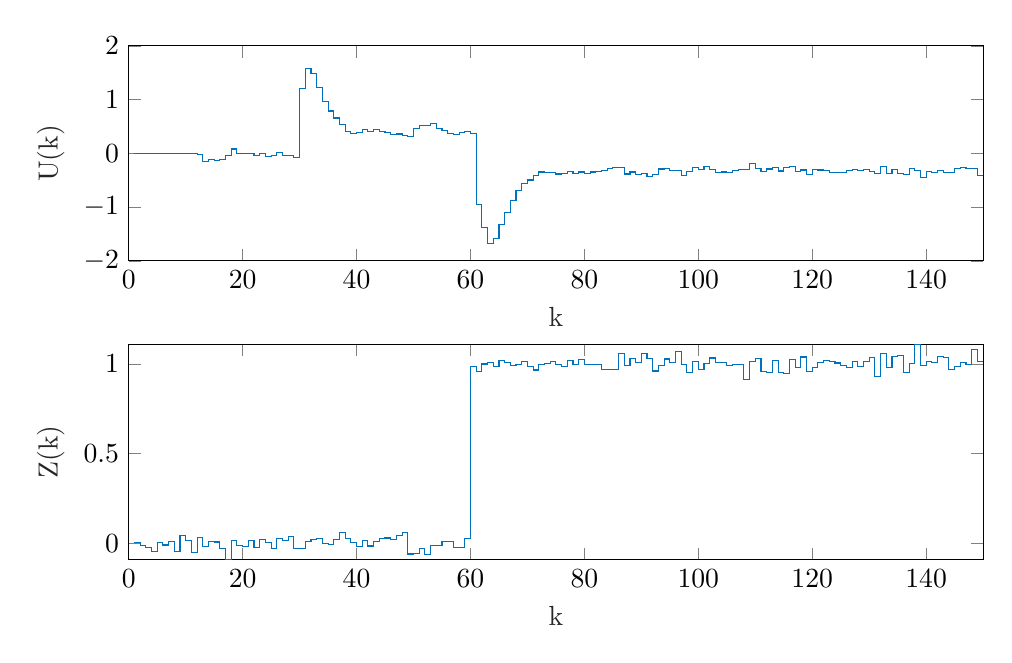
\begin{tikzpicture}

\begin{axis}[%
width=4.272in,
height=1.075in,
at={(0.717in,1.839in)},
scale only axis,
xmin=0,
xmax=150,
xlabel style={font=\color{white!15!black}},
xlabel={k},
ymin=-2,
ymax=2,
ylabel style={font=\color{white!15!black}},
ylabel={U(k)},
axis background/.style={fill=white}
]
\addplot[const plot, color=mycolor1, forget plot] table[row sep=crcr] {%
1	0\\
2	0\\
3	0\\
4	0\\
5	0\\
6	0\\
7	0\\
8	0\\
9	0\\
10	0\\
11	0\\
12	-0.0207382081833764\\
13	-0.150432916805117\\
14	-0.114070412292392\\
15	-0.138032119929149\\
16	-0.110391106356429\\
17	-0.0431938125308523\\
18	0.0797813120368421\\
19	-0.00944898217595301\\
20	0.00456197375392563\\
21	-0.00695559106065184\\
22	-0.0451516513854095\\
23	-0.00646889274841674\\
24	-0.0539562735266854\\
25	-0.0368217345473017\\
26	0.0130420142416154\\
27	-0.0391470699739274\\
28	-0.0337711227747506\\
29	-0.0767037352864819\\
30	1.21373363251892\\
31	1.57748369278364\\
32	1.48095697505767\\
33	1.23239760371956\\
34	0.965264569524801\\
35	0.78700451885889\\
36	0.657011962703161\\
37	0.5296538716866\\
38	0.398211352879038\\
39	0.375439470154172\\
40	0.390933765790895\\
41	0.436108684798621\\
42	0.41142157748765\\
43	0.444477099931547\\
44	0.412992779877918\\
45	0.381775732295022\\
46	0.356663107299105\\
47	0.360179084609673\\
48	0.331236901537313\\
49	0.307724410358705\\
50	0.460525703942413\\
51	0.513032615018699\\
52	0.516554998067525\\
53	0.546637263055875\\
54	0.465435514295844\\
55	0.43040341765487\\
56	0.37411819002623\\
57	0.353172247727878\\
58	0.388731800972962\\
59	0.413840222492077\\
60	0.364286385302505\\
61	-0.959572713123259\\
62	-1.37994755207964\\
63	-1.68144536778805\\
64	-1.58006818029631\\
65	-1.32015769827486\\
66	-1.10120471553292\\
67	-0.870263517923897\\
68	-0.684850688473676\\
69	-0.560558119141631\\
70	-0.496730856878388\\
71	-0.414437351644308\\
72	-0.348298439356271\\
73	-0.350090895267608\\
74	-0.358836400578496\\
75	-0.385575245419159\\
76	-0.371403605461378\\
77	-0.34544005808155\\
78	-0.372956572310239\\
79	-0.34744569964781\\
80	-0.382741222153163\\
81	-0.348384261431197\\
82	-0.342292096887487\\
83	-0.327011306062553\\
84	-0.286154383983979\\
85	-0.271788415741227\\
86	-0.2634446352335\\
87	-0.384748744347855\\
88	-0.347194507711677\\
89	-0.39789740540123\\
90	-0.368587140969201\\
91	-0.424601567733075\\
92	-0.393747590837207\\
93	-0.292693237433872\\
94	-0.281716595960061\\
95	-0.318092044014778\\
96	-0.319540562703438\\
97	-0.416262590092689\\
98	-0.345351935936652\\
99	-0.262828953110771\\
100	-0.298684929631751\\
101	-0.24942050446522\\
102	-0.294890367258289\\
103	-0.351209752120924\\
104	-0.348552890853989\\
105	-0.351467534436577\\
106	-0.320746898334297\\
107	-0.309220608450862\\
108	-0.303580928067648\\
109	-0.188390491314248\\
110	-0.288484794145148\\
111	-0.341019950878359\\
112	-0.291150489258594\\
113	-0.264257216888345\\
114	-0.329378070976033\\
115	-0.264607516046224\\
116	-0.250613530565349\\
117	-0.337919560525971\\
118	-0.311357889828788\\
119	-0.400307683501854\\
120	-0.307759341072966\\
121	-0.310371838779431\\
122	-0.326632813816994\\
123	-0.352409216174631\\
124	-0.363260027512877\\
125	-0.352774553668663\\
126	-0.32480438652277\\
127	-0.294235830839643\\
128	-0.325725175000938\\
129	-0.299975270910756\\
130	-0.334393017655264\\
131	-0.369462917243658\\
132	-0.243537046623792\\
133	-0.373960205529092\\
134	-0.295095181233656\\
135	-0.380638280158422\\
136	-0.401258399301341\\
137	-0.288741464720124\\
138	-0.313339344893201\\
139	-0.442352490034343\\
140	-0.345513088530733\\
141	-0.356197244853887\\
142	-0.319583721356274\\
143	-0.352253693563447\\
144	-0.356821286455329\\
145	-0.277038060540829\\
146	-0.267270797767871\\
147	-0.287436450591829\\
148	-0.289869847560188\\
149	-0.413062331101117\\
150	-0.365360087195853\\
};
\end{axis}

\begin{axis}[%
width=4.272in,
height=1.075in,
at={(0.717in,0.346in)},
scale only axis,
xmin=0,
xmax=150,
xlabel style={font=\color{white!15!black}},
xlabel={k},
ymin=-0.0904854053555337,
ymax=1.10961276291618,
ylabel style={font=\color{white!15!black}},
ylabel={Z(k)},
axis background/.style={fill=white}
]
\addplot[const plot, color=mycolor1, forget plot] table[row sep=crcr] {%
1	0.00320109444637361\\
2	-0.0114697652482808\\
3	-0.0233637874729122\\
4	-0.0467967259443988\\
5	0.00485004057057498\\
6	-0.0100249726914904\\
7	0.010085080649941\\
8	-0.0460600473605885\\
9	0.0418000771575006\\
10	0.0154067412766389\\
11	-0.0495410718950959\\
12	0.0334271605009296\\
13	-0.0185808413973367\\
14	0.00955708670807528\\
15	0.00694001008150868\\
16	-0.0277711572444773\\
17	-0.0904854053555337\\
18	0.0169357455017639\\
19	-0.0108161694404724\\
20	-0.0189059570026563\\
21	0.0132471829936653\\
22	-0.0218096193595153\\
23	0.0212249243557949\\
24	0.00477179668375428\\
25	-0.0313482556361717\\
26	0.0264628864912442\\
27	0.015005291161245\\
28	0.0395969610936456\\
29	-0.0282272068295588\\
30	-0.0283110569525606\\
31	0.00990823580967339\\
32	0.0210934406447205\\
33	0.0261873447336513\\
34	0.000205841451220666\\
35	-0.00745956625213493\\
36	0.0206440156465603\\
37	0.0621239727398428\\
38	0.0279730077032093\\
39	0.00267329330820531\\
40	-0.0181677298137033\\
41	0.0158035025525493\\
42	-0.0153087279055083\\
43	0.0075403130677599\\
44	0.0246103686996763\\
45	0.0292280764443272\\
46	0.0185985538746858\\
47	0.0435741078198438\\
48	0.0585402400337738\\
49	-0.0600094290057894\\
50	-0.0562469324408757\\
51	-0.029176477708716\\
52	-0.063180001832008\\
53	-0.011292495349813\\
54	-0.0106379260786009\\
55	0.00791916560463933\\
56	0.00904923387261777\\
57	-0.0216985553405167\\
58	-0.025719262352857\\
59	0.0250895918737771\\
60	0.987921830560224\\
61	0.956638716851639\\
62	1.00032595032863\\
63	1.00645522207993\\
64	0.987002232235905\\
65	1.02098364693596\\
66	1.00713985815599\\
67	0.993269309782233\\
68	0.998607504598126\\
69	1.01448898142715\\
70	0.98604115684184\\
71	0.966639655474745\\
72	0.995079993718909\\
73	1.0040840140282\\
74	1.01610953819819\\
75	0.999047410356347\\
76	0.985536850370828\\
77	1.01885778827324\\
78	0.996409915324052\\
79	1.0255203528016\\
80	0.997160188027999\\
81	0.99980102553007\\
82	0.997095110508513\\
83	0.970867887605604\\
84	0.970687218744004\\
85	0.969603533400639\\
86	1.05644127526651\\
87	0.993669468410765\\
88	1.02973842765711\\
89	1.01104129284893\\
90	1.05879560558852\\
91	1.02931658990097\\
92	0.961199996468672\\
93	0.989651789764824\\
94	1.02819633493728\\
95	1.00911322815705\\
96	1.07163176915501\\
97	0.998485574778364\\
98	0.950925749244625\\
99	1.01404314736891\\
100	0.971165755357454\\
101	1.0015632608155\\
102	1.03409080386578\\
103	1.00974546808027\\
104	1.00947540269712\\
105	0.993763404838673\\
106	0.995369716113573\\
107	0.99674061291084\\
108	0.911488419214795\\
109	1.01243645303507\\
110	1.03131436448876\\
111	0.958965244354826\\
112	0.951871134492461\\
113	1.01963810184937\\
114	0.952327950068639\\
115	0.946892641354316\\
116	1.02494961813974\\
117	0.97930977507839\\
118	1.03936728978602\\
119	0.959135011003551\\
120	0.980572468971941\\
121	1.00764307367438\\
122	1.01737194538327\\
123	1.01478789555557\\
124	1.00605440203498\\
125	0.992732929221832\\
126	0.981683555267178\\
127	1.01519414892686\\
128	0.987767277784009\\
129	1.01333265407652\\
130	1.03439627926951\\
131	0.928869879872464\\
132	1.05706267233577\\
133	0.980012495822449\\
134	1.04163006379163\\
135	1.0490656490426\\
136	0.953549047194403\\
137	1.00559528210681\\
138	1.10961276291618\\
139	0.993212907040124\\
140	1.01537760486832\\
141	1.01046350622815\\
142	1.04009458425805\\
143	1.0344850871029\\
144	0.970070603784824\\
145	0.986133439541569\\
146	1.01085359064413\\
147	0.998153122899923\\
148	1.08016293824117\\
149	1.01387118668564\\
150	1.01383552505555\\
};
\end{axis}
\end{tikzpicture}%
\caption{Zakłócenie i sygnał sterujący- szum średni}
\end{figure}

\begin{figure}[H]
\centering
% This file was created by matlab2tikz.
%
%The latest updates can be retrieved from
%  http://www.mathworks.com/matlabcentral/fileexchange/22022-matlab2tikz-matlab2tikz
%where you can also make suggestions and rate matlab2tikz.
%
\definecolor{mycolor1}{rgb}{0.00000,0.44700,0.74100}%
\definecolor{mycolor2}{rgb}{0.85000,0.32500,0.09800}%
%
\begin{tikzpicture}

\begin{axis}[%
width=4.272in,
height=2.472in,
at={(0.717in,0.441in)},
scale only axis,
xmin=0,
xmax=150,
xlabel style={font=\color{white!15!black}},
xlabel={k},
ymin=-0.5,
ymax=2,
ylabel style={font=\color{white!15!black}},
ylabel={Y(k)},
axis background/.style={fill=white},
legend style={legend cell align=left, align=left, draw=white!15!black}
]
\addplot[const plot, color=mycolor1] table[row sep=crcr] {%
1	0\\
2	0\\
3	0\\
4	0\\
5	0\\
6	0\\
7	0\\
8	0\\
9	0\\
10	0\\
11	0\\
12	0.0171990847891853\\
13	0.0266177756528847\\
14	0.02137108233\\
15	0.0330158905340646\\
16	0.0324154589389564\\
17	0.0371607688283554\\
18	0.0404626751668299\\
19	0.0329553325173019\\
20	-0.00605902650916875\\
21	-0.0151039519800049\\
22	-0.0333982298619926\\
23	-0.0484223791249575\\
24	-0.0462738924633196\\
25	-0.0336265428977369\\
26	-0.0262778180342901\\
27	-0.0211200895598107\\
28	-0.0255391325954317\\
29	-0.0235197344379676\\
30	-0.0187037173571748\\
31	-0.0165391897810835\\
32	-0.0262112161834222\\
33	-0.0277067475770525\\
34	-0.0288902506664775\\
35	-0.0271630677753391\\
36	-0.0311678044101274\\
37	0.150316023674103\\
38	0.373281883540571\\
39	0.574516220712918\\
40	0.735215261270069\\
41	0.83933500007451\\
42	0.90559530621634\\
43	0.94457176626247\\
44	0.969557330223427\\
45	0.967231763384215\\
46	0.966529086741118\\
47	0.971573194276677\\
48	0.983718344775683\\
49	0.989107067752872\\
50	1.00401198537534\\
51	1.0160467805734\\
52	0.998327457122411\\
53	0.979551505913913\\
54	0.968588481249788\\
55	0.947467851627694\\
56	0.935271690561167\\
57	0.946563984315869\\
58	0.968727846062358\\
59	0.990153202918692\\
60	1.00837889616589\\
61	1.01288522341163\\
62	1.02241153478458\\
63	1.21719747237203\\
64	1.38039304961991\\
65	1.53889774363332\\
66	1.68440934385087\\
67	1.80238142053909\\
68	1.71786259087622\\
69	1.56716414204696\\
70	1.37262598736424\\
71	1.20105450105281\\
72	1.07712637127835\\
73	0.983305975194058\\
74	0.922149803219423\\
75	0.895214852857951\\
76	0.887493167135894\\
77	0.889709116282479\\
78	0.898267838737148\\
79	0.911557350450668\\
80	0.929060880476776\\
81	0.938041587074719\\
82	0.947185498513306\\
83	0.950748823501142\\
84	0.957530080831976\\
85	0.958427531594741\\
86	0.95700564557366\\
87	0.950035674239705\\
88	0.948008085076292\\
89	0.964261224693255\\
90	0.967948732692378\\
91	0.9843696700401\\
92	0.997444516844014\\
93	1.0201864547535\\
94	1.01678567705152\\
95	1.0048935106127\\
96	0.992254306595325\\
97	0.992445312152983\\
98	0.980038591091436\\
99	0.985366065517575\\
100	0.989703804899045\\
101	0.985836683011232\\
102	0.990112515399646\\
103	0.985064027097679\\
104	0.972438504946846\\
105	0.977546687893186\\
106	0.989225862678535\\
107	0.994751727026012\\
108	1.00397123970342\\
109	1.00633343913586\\
110	1.00056522369379\\
111	0.978348292018517\\
112	0.978357882144549\\
113	0.986484264937203\\
114	0.980803259913713\\
115	0.975266367425932\\
116	1.00121925362521\\
117	0.996897628487367\\
118	0.984386038085821\\
119	0.996191177563293\\
120	1.00160152632388\\
121	1.00928134177887\\
122	1.00930998833365\\
123	1.01609405446809\\
124	1.01512157062821\\
125	1.01988736080289\\
126	1.01040197821745\\
127	1.01316745865777\\
128	1.01257884513284\\
129	1.00743077854999\\
130	1.00570171711401\\
131	0.996709308825152\\
132	0.995062927201976\\
133	1.0017189157352\\
134	0.99079146494102\\
135	1.00253503477304\\
136	1.00114733093277\\
137	1.00742346582271\\
138	1.00918214072249\\
139	1.0096726112476\\
140	1.00194998903748\\
141	1.02732573648675\\
142	1.01388814450321\\
143	1.00290455384572\\
144	1.00818433807832\\
145	1.01552320587371\\
146	1.0019189019121\\
147	0.990224212086093\\
148	0.981396554017562\\
149	0.983780320622568\\
150	0.978610045034473\\
};
\addlegendentry{Y}

\addplot[const plot, color=mycolor2] table[row sep=crcr] {%
1	0\\
2	0\\
3	0\\
4	0\\
5	0\\
6	0\\
7	0\\
8	0\\
9	0\\
10	0\\
11	0\\
12	0\\
13	0\\
14	0\\
15	0\\
16	0\\
17	0\\
18	0\\
19	0\\
20	0\\
21	0\\
22	0\\
23	0\\
24	0\\
25	0\\
26	0\\
27	0\\
28	0\\
29	0\\
30	1\\
31	1\\
32	1\\
33	1\\
34	1\\
35	1\\
36	1\\
37	1\\
38	1\\
39	1\\
40	1\\
41	1\\
42	1\\
43	1\\
44	1\\
45	1\\
46	1\\
47	1\\
48	1\\
49	1\\
50	1\\
51	1\\
52	1\\
53	1\\
54	1\\
55	1\\
56	1\\
57	1\\
58	1\\
59	1\\
60	1\\
61	1\\
62	1\\
63	1\\
64	1\\
65	1\\
66	1\\
67	1\\
68	1\\
69	1\\
70	1\\
71	1\\
72	1\\
73	1\\
74	1\\
75	1\\
76	1\\
77	1\\
78	1\\
79	1\\
80	1\\
81	1\\
82	1\\
83	1\\
84	1\\
85	1\\
86	1\\
87	1\\
88	1\\
89	1\\
90	1\\
91	1\\
92	1\\
93	1\\
94	1\\
95	1\\
96	1\\
97	1\\
98	1\\
99	1\\
100	1\\
101	1\\
102	1\\
103	1\\
104	1\\
105	1\\
106	1\\
107	1\\
108	1\\
109	1\\
110	1\\
111	1\\
112	1\\
113	1\\
114	1\\
115	1\\
116	1\\
117	1\\
118	1\\
119	1\\
120	1\\
121	1\\
122	1\\
123	1\\
124	1\\
125	1\\
126	1\\
127	1\\
128	1\\
129	1\\
130	1\\
131	1\\
132	1\\
133	1\\
134	1\\
135	1\\
136	1\\
137	1\\
138	1\\
139	1\\
140	1\\
141	1\\
142	1\\
143	1\\
144	1\\
145	1\\
146	1\\
147	1\\
148	1\\
149	1\\
150	1\\
};
\addlegendentry{Yzad}

\end{axis}
\end{tikzpicture}%
\caption{Wyjście dla pomiaru z szumem średnim ($E=11,5103$)}
\end{figure}

\begin{figure}[H]
\centering
% This file was created by matlab2tikz.
%
%The latest updates can be retrieved from
%  http://www.mathworks.com/matlabcentral/fileexchange/22022-matlab2tikz-matlab2tikz
%where you can also make suggestions and rate matlab2tikz.
%
\definecolor{mycolor1}{rgb}{0.00000,0.44700,0.74100}%
%
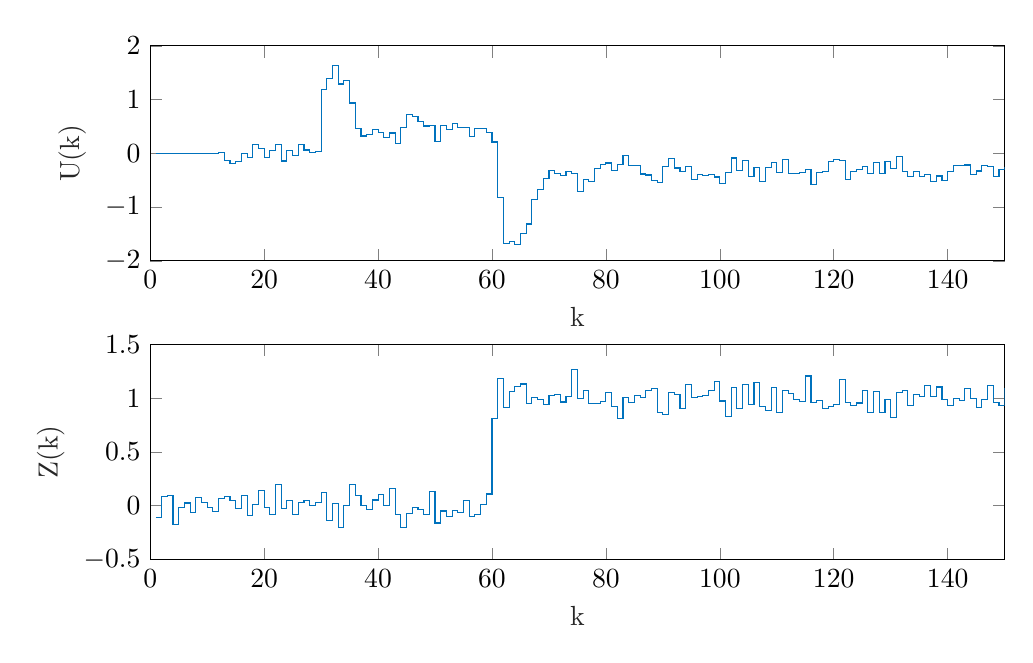
\begin{tikzpicture}

\begin{axis}[%
width=4.272in,
height=1.075in,
at={(0.717in,1.839in)},
scale only axis,
xmin=0,
xmax=150,
xlabel style={font=\color{white!15!black}},
xlabel={k},
ymin=-2,
ymax=2,
ylabel style={font=\color{white!15!black}},
ylabel={U(k)},
axis background/.style={fill=white}
]
\addplot[const plot, color=mycolor1, forget plot] table[row sep=crcr] {%
1	0\\
2	0\\
3	0\\
4	0\\
5	0\\
6	0\\
7	0\\
8	0\\
9	0\\
10	0\\
11	0\\
12	0.0112425860890454\\
13	-0.134335630286902\\
14	-0.185045568518065\\
15	-0.148969857682414\\
16	-0.00778489127349916\\
17	-0.0798120707501585\\
18	0.168225965498215\\
19	0.0916188978007313\\
20	-0.0722220242536749\\
21	0.0488008242735829\\
22	0.157855233346119\\
23	-0.14343327770835\\
24	0.0485039224786061\\
25	-0.036433576777133\\
26	0.159209827827496\\
27	0.0614319283106867\\
28	0.0173049608605574\\
29	0.0274095848003943\\
30	1.18800891525148\\
31	1.39617777178007\\
32	1.62922510713003\\
33	1.28986655541941\\
34	1.35891255938908\\
35	0.935995406690737\\
36	0.469266698185795\\
37	0.322647217669518\\
38	0.346646968394453\\
39	0.439481590846806\\
40	0.383268976338592\\
41	0.29246655266858\\
42	0.378859856495124\\
43	0.188892888667748\\
44	0.481935715401568\\
45	0.720550524607832\\
46	0.685009550176658\\
47	0.58625293701548\\
48	0.507770320014285\\
49	0.514059524170595\\
50	0.218170282437539\\
51	0.52232717212534\\
52	0.441860520138361\\
53	0.549217217809028\\
54	0.484277650711196\\
55	0.487961036977969\\
56	0.315620041316605\\
57	0.463722316937533\\
58	0.469563196132282\\
59	0.385209462770834\\
60	0.211458975380797\\
61	-0.825004355989058\\
62	-1.67574931700302\\
63	-1.64744814659328\\
64	-1.70431257042004\\
65	-1.49705972092496\\
66	-1.31556071724992\\
67	-0.862469776720799\\
68	-0.668809946507051\\
69	-0.469803098242145\\
70	-0.325456185604305\\
71	-0.38051458905945\\
72	-0.405580506298859\\
73	-0.339171685398677\\
74	-0.377086900847224\\
75	-0.716884446783785\\
76	-0.47952262596985\\
77	-0.519355939344809\\
78	-0.286475788211918\\
79	-0.203560385957308\\
80	-0.180104773190205\\
81	-0.314871862531214\\
82	-0.200695103851073\\
83	-0.0446848487364954\\
84	-0.226872081824324\\
85	-0.227909739842205\\
86	-0.385460509166599\\
87	-0.404143824506832\\
88	-0.504956316605368\\
89	-0.543708896569871\\
90	-0.248730616515689\\
91	-0.0986080827279952\\
92	-0.273307648067015\\
93	-0.331234728112738\\
94	-0.240730553960417\\
95	-0.493556243582254\\
96	-0.3905477114633\\
97	-0.404702650281956\\
98	-0.386926224472736\\
99	-0.440253112053931\\
100	-0.560964585240496\\
101	-0.360407559509751\\
102	-0.0869393599737121\\
103	-0.317085738279582\\
104	-0.127496509147312\\
105	-0.434716433423199\\
106	-0.259673126767248\\
107	-0.527315558228875\\
108	-0.263381428304811\\
109	-0.164467451986712\\
110	-0.356687009522812\\
111	-0.121607283387638\\
112	-0.369739278801802\\
113	-0.38016696499471\\
114	-0.35377025773657\\
115	-0.300767382387272\\
116	-0.588148930610815\\
117	-0.354436484801845\\
118	-0.332427800988533\\
119	-0.153982462540731\\
120	-0.118618852659075\\
121	-0.139898322557044\\
122	-0.486342661443302\\
123	-0.345015415514119\\
124	-0.293435759928378\\
125	-0.245055120585917\\
126	-0.382851551399373\\
127	-0.169932737664176\\
128	-0.382457292254044\\
129	-0.150301432642932\\
130	-0.278191793922966\\
131	-0.0558911232996129\\
132	-0.336204839271164\\
133	-0.434759615018006\\
134	-0.338575738115096\\
135	-0.425213763737322\\
136	-0.391166853208026\\
137	-0.528851296081234\\
138	-0.422015803888237\\
139	-0.511183118717043\\
140	-0.346263757709117\\
141	-0.223641003158337\\
142	-0.234058590141052\\
143	-0.218144794915123\\
144	-0.389034907091786\\
145	-0.328177551380401\\
146	-0.221278387779689\\
147	-0.250964604463829\\
148	-0.435785062092553\\
149	-0.308901906226218\\
150	-0.252937633039795\\
};
\end{axis}

\begin{axis}[%
width=4.272in,
height=1.075in,
at={(0.717in,0.346in)},
scale only axis,
xmin=0,
xmax=150,
xlabel style={font=\color{white!15!black}},
xlabel={k},
ymin=-0.5,
ymax=1.5,
ylabel style={font=\color{white!15!black}},
ylabel={Z(k)},
axis background/.style={fill=white}
]
\addplot[const plot, color=mycolor1, forget plot] table[row sep=crcr] {%
1	-0.107409163637826\\
2	0.0869552807313267\\
3	0.0981051414525262\\
4	-0.175882536913901\\
5	-0.0148095957567039\\
6	0.0251941746175391\\
7	-0.0610384625892835\\
8	0.0760979810218383\\
9	0.025442950225039\\
10	-0.0152833676937382\\
11	-0.0557410875209181\\
12	0.0677017656847446\\
13	0.0849297440422057\\
14	0.0469307182589951\\
15	-0.0239781704489258\\
16	0.0920985453809901\\
17	-0.0906881378407088\\
18	0.014444060627547\\
19	0.13964090281818\\
20	-0.0189698759604886\\
21	-0.0843835890826002\\
22	0.194343804984731\\
23	-0.0246921540574881\\
24	0.0441619155865907\\
25	-0.0803611484220362\\
26	0.0287609432704476\\
27	0.0467018093753898\\
28	0.000456160956191707\\
29	0.0326090358603265\\
30	0.120458671653349\\
31	-0.140411583207086\\
32	0.0205563555454331\\
33	-0.199119578942207\\
34	0.00284089339182698\\
35	0.193051540875233\\
36	0.0941136788326655\\
37	-0.000692445130187209\\
38	-0.0338241647272311\\
39	0.0528265783681366\\
40	0.105689959434016\\
41	0.00147406166024418\\
42	0.161476126691229\\
43	-0.0815854961856177\\
44	-0.199775912436652\\
45	-0.0748191408314749\\
46	-0.0199304020638472\\
47	-0.0372760077970442\\
48	-0.0847371160164792\\
49	0.133723804312817\\
50	-0.161631725794785\\
51	-0.0491817594931569\\
52	-0.0969301567007431\\
53	-0.0474107920526903\\
54	-0.066616382519409\\
55	0.0478374683115003\\
56	-0.104105813301215\\
57	-0.0820659090657572\\
58	0.010112960601311\\
59	0.108398253686458\\
60	0.814547276261703\\
61	1.17997527857881\\
62	0.912162569442147\\
63	1.06477327264332\\
64	1.10495650322525\\
65	1.13230933768457\\
66	0.948264103436202\\
67	1.00243149497111\\
68	0.983763312644646\\
69	0.939433891393262\\
70	1.0271709764009\\
71	1.03586434121791\\
72	0.964768487721931\\
73	1.01323599281997\\
74	1.26735817771994\\
75	0.999243392455546\\
76	1.07103029366614\\
77	0.95374606371871\\
78	0.947212209939989\\
79	0.96542129330955\\
80	1.05645577737344\\
81	0.919846085599793\\
82	0.814705321483177\\
83	1.00532160174532\\
84	0.956358478294511\\
85	1.02800074722662\\
86	1.00846058871809\\
87	1.07291190595681\\
88	1.09007530956458\\
89	0.867436170546814\\
90	0.847542117151499\\
91	1.05024333330629\\
92	1.03063914256495\\
93	0.906083953468134\\
94	1.12374021264301\\
95	1.0033011914555\\
96	1.01235683182212\\
97	1.02739393795508\\
98	1.07541658082824\\
99	1.15244975057338\\
100	0.97380242377443\\
101	0.826931649222705\\
102	1.10134642999901\\
103	0.90722639015537\\
104	1.12436802862236\\
105	0.941051130241411\\
106	1.14914817347865\\
107	0.919402190528573\\
108	0.88874009472468\\
109	1.09569395680994\\
110	0.863694841106271\\
111	1.06805849627241\\
112	1.04378236225657\\
113	0.985673245332796\\
114	0.965846749539944\\
115	1.20578106340642\\
116	0.96254649645742\\
117	0.980979680254716\\
118	0.90612675893883\\
119	0.918653763561683\\
120	0.94163812484714\\
121	1.17095253705239\\
122	0.960958018222896\\
123	0.93099346367202\\
124	0.955177929807091\\
125	1.07143763500996\\
126	0.868426875171689\\
127	1.06271220952632\\
128	0.866870515673932\\
129	0.986915184824033\\
130	0.817310382928203\\
131	1.05359224651102\\
132	1.06928647154366\\
133	0.931245024491926\\
134	1.03175757564404\\
135	1.01628423401243\\
136	1.11591159058306\\
137	1.01283880586636\\
138	1.10394581333017\\
139	0.988322885869547\\
140	0.935170308989575\\
141	0.996201879511236\\
142	0.980067518122789\\
143	1.08816698720157\\
144	0.994385592909307\\
145	0.91587611306126\\
146	0.984515616191396\\
147	1.11885946704643\\
148	0.958509272076415\\
149	0.93413832374886\\
150	1.09839906680987\\
};
\end{axis}
\end{tikzpicture}%
\caption{Zakłócenie i sygnał sterujący- szum duży}
\end{figure}s

\begin{figure}[H]
\centering
% This file was created by matlab2tikz.
%
%The latest updates can be retrieved from
%  http://www.mathworks.com/matlabcentral/fileexchange/22022-matlab2tikz-matlab2tikz
%where you can also make suggestions and rate matlab2tikz.
%
\definecolor{mycolor1}{rgb}{0.00000,0.44700,0.74100}%
\definecolor{mycolor2}{rgb}{0.85000,0.32500,0.09800}%
%
\begin{tikzpicture}

\begin{axis}[%
width=4.272in,
height=2.472in,
at={(0.717in,0.441in)},
scale only axis,
xmin=0,
xmax=150,
xlabel style={font=\color{white!15!black}},
xlabel={k},
ymin=-0.5,
ymax=2,
ylabel style={font=\color{white!15!black}},
ylabel={Y(k)},
axis background/.style={fill=white},
legend style={legend cell align=left, align=left, draw=white!15!black}
]
\addplot[const plot, color=mycolor1] table[row sep=crcr] {%
1	0\\
2	0\\
3	0\\
4	0\\
5	0\\
6	0\\
7	0\\
8	0\\
9	0\\
10	0\\
11	0\\
12	-0.00932395844835842\\
13	-0.0249732779094304\\
14	-0.0462342044946201\\
15	-0.0394131167562775\\
16	-0.0291642737086906\\
17	-0.0270716378804508\\
18	-0.0389079290265876\\
19	-0.0237096208524286\\
20	-0.0680251452328963\\
21	-0.0941598500406067\\
22	-0.0876328565079645\\
23	-0.0935652445106375\\
24	-0.122120161703767\\
25	-0.0545026504073886\\
26	-0.0481277018515096\\
27	-0.0515769869832808\\
28	-0.0620447344680745\\
29	-0.0323542221421181\\
30	-0.0453076857955384\\
31	-0.0386061143866624\\
32	-0.0380067986111862\\
33	0.00921090013668197\\
34	-0.0144914019676052\\
35	-0.00885789766551821\\
36	-0.0464455309252497\\
37	0.13297299082672\\
38	0.370901422819155\\
39	0.607109819388092\\
40	0.759182029522761\\
41	0.906059647050559\\
42	0.999818235608636\\
43	1.02930036567269\\
44	1.0133928124681\\
45	1.0346099991438\\
46	1.01775708565466\\
47	0.971039108631479\\
48	0.941347523001663\\
49	0.93811006122794\\
50	0.90361818161633\\
51	0.905235143127714\\
52	0.98696843462076\\
53	0.997301235423661\\
54	1.01684547763088\\
55	1.01429385710134\\
56	1.02361710569762\\
57	0.984922969422167\\
58	1.01697802135786\\
59	1.00363117492976\\
60	1.01222388560274\\
61	1.02981919645092\\
62	1.06622269235514\\
63	1.21609940324224\\
64	1.44389197096283\\
65	1.59310791507708\\
66	1.74419294506313\\
67	1.86032609303669\\
68	1.81392109315252\\
69	1.59995403299167\\
70	1.40925750005798\\
71	1.21307409297356\\
72	1.04631950723299\\
73	0.931034447578793\\
74	0.887760085140817\\
75	0.858057405998818\\
76	0.867196126012618\\
77	0.946060309614897\\
78	0.953079344392279\\
79	0.969027878998427\\
80	0.968101864843424\\
81	0.959734070119015\\
82	0.904855290162109\\
83	0.906136025538982\\
84	0.872360881053454\\
85	0.853922817034791\\
86	0.888596763219179\\
87	0.913862620448574\\
88	0.931873100899753\\
89	0.960717239557309\\
90	1.02323336062518\\
91	1.05725092730242\\
92	1.0427649655828\\
93	1.0029984142548\\
94	1.00503361227126\\
95	0.987027109732246\\
96	0.938468989841496\\
97	0.981069879603072\\
98	1.01729944192638\\
99	1.02714353245808\\
100	1.03057033442649\\
101	1.05644674305273\\
102	1.05806652873783\\
103	1.03710955752334\\
104	0.986102154962403\\
105	0.998174510744007\\
106	0.96125995860391\\
107	0.953588397585833\\
108	0.937593852028579\\
109	1.00574605035219\\
110	0.987824629558798\\
111	0.993855231443089\\
112	0.997165568239598\\
113	0.978197916007305\\
114	0.963569927369103\\
115	0.983085608300769\\
116	1.00384045785411\\
117	0.991119910303568\\
118	1.06276367671565\\
119	1.04209636634061\\
120	1.02545433606755\\
121	0.998932304082016\\
122	0.985464813917983\\
123	0.935796250662267\\
124	0.970470217009051\\
125	0.961922353460384\\
126	0.974689495219506\\
127	0.997557684545838\\
128	1.03981104821058\\
129	0.986426770771076\\
130	0.997736087793388\\
131	0.97558651548887\\
132	0.987495391306278\\
133	0.943962709221018\\
134	0.983960132587423\\
135	0.992338305008809\\
136	1.00561420603782\\
137	1.02004356413493\\
138	1.06277459564718\\
139	1.08128952777417\\
140	1.06192401049158\\
141	1.07620703859273\\
142	1.05238516694692\\
143	1.02454272298809\\
144	0.991128762126001\\
145	0.972299083403783\\
146	0.963468562227888\\
147	0.959651428865378\\
148	0.958492846141326\\
149	0.970711677462253\\
150	1.01183763005872\\
};
\addlegendentry{Y}

\addplot[const plot, color=mycolor2] table[row sep=crcr] {%
1	0\\
2	0\\
3	0\\
4	0\\
5	0\\
6	0\\
7	0\\
8	0\\
9	0\\
10	0\\
11	0\\
12	0\\
13	0\\
14	0\\
15	0\\
16	0\\
17	0\\
18	0\\
19	0\\
20	0\\
21	0\\
22	0\\
23	0\\
24	0\\
25	0\\
26	0\\
27	0\\
28	0\\
29	0\\
30	1\\
31	1\\
32	1\\
33	1\\
34	1\\
35	1\\
36	1\\
37	1\\
38	1\\
39	1\\
40	1\\
41	1\\
42	1\\
43	1\\
44	1\\
45	1\\
46	1\\
47	1\\
48	1\\
49	1\\
50	1\\
51	1\\
52	1\\
53	1\\
54	1\\
55	1\\
56	1\\
57	1\\
58	1\\
59	1\\
60	1\\
61	1\\
62	1\\
63	1\\
64	1\\
65	1\\
66	1\\
67	1\\
68	1\\
69	1\\
70	1\\
71	1\\
72	1\\
73	1\\
74	1\\
75	1\\
76	1\\
77	1\\
78	1\\
79	1\\
80	1\\
81	1\\
82	1\\
83	1\\
84	1\\
85	1\\
86	1\\
87	1\\
88	1\\
89	1\\
90	1\\
91	1\\
92	1\\
93	1\\
94	1\\
95	1\\
96	1\\
97	1\\
98	1\\
99	1\\
100	1\\
101	1\\
102	1\\
103	1\\
104	1\\
105	1\\
106	1\\
107	1\\
108	1\\
109	1\\
110	1\\
111	1\\
112	1\\
113	1\\
114	1\\
115	1\\
116	1\\
117	1\\
118	1\\
119	1\\
120	1\\
121	1\\
122	1\\
123	1\\
124	1\\
125	1\\
126	1\\
127	1\\
128	1\\
129	1\\
130	1\\
131	1\\
132	1\\
133	1\\
134	1\\
135	1\\
136	1\\
137	1\\
138	1\\
139	1\\
140	1\\
141	1\\
142	1\\
143	1\\
144	1\\
145	1\\
146	1\\
147	1\\
148	1\\
149	1\\
150	1\\
};
\addlegendentry{Yzad}

\end{axis}
\end{tikzpicture}%
\caption{Wyjście dla pomiaru z szumem dużym (błąd $E=12,1956$)}
\end{figure}


\section{Szum nałożony na zakłócenie sinusoidalne}

\begin{figure}[H]
\centering
% This file was created by matlab2tikz.
%
%The latest updates can be retrieved from
%  http://www.mathworks.com/matlabcentral/fileexchange/22022-matlab2tikz-matlab2tikz
%where you can also make suggestions and rate matlab2tikz.
%
\definecolor{mycolor1}{rgb}{0.00000,0.44700,0.74100}%
%
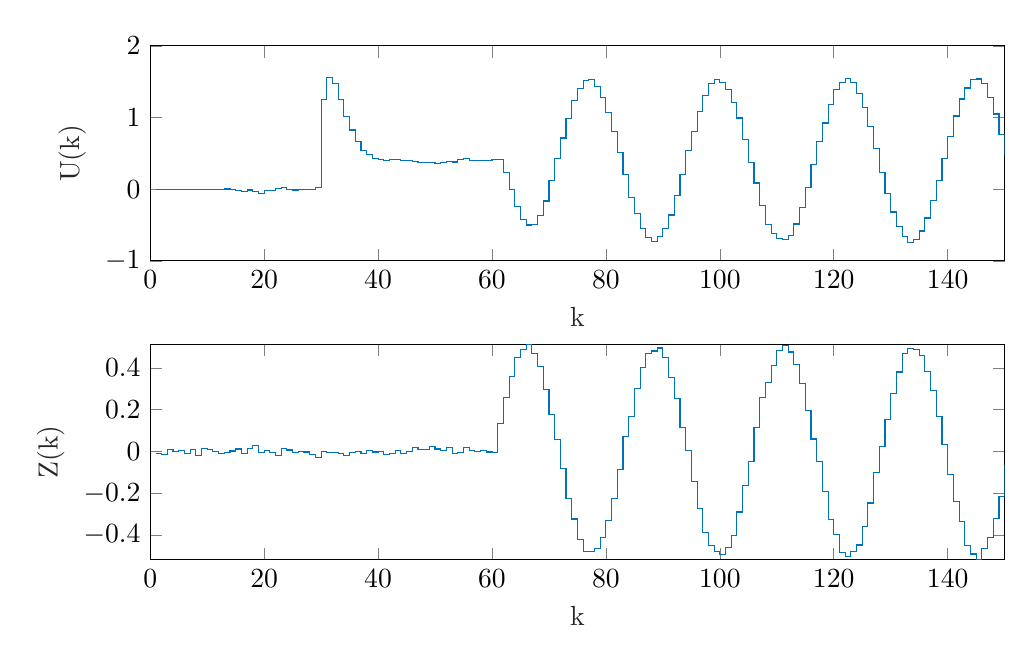
\begin{tikzpicture}

\begin{axis}[%
width=4.272in,
height=1.075in,
at={(0.717in,1.839in)},
scale only axis,
xmin=0,
xmax=150,
xlabel style={font=\color{white!15!black}},
xlabel={k},
ymin=-1,
ymax=2,
ylabel style={font=\color{white!15!black}},
ylabel={U(k)},
axis background/.style={fill=white}
]
\addplot[const plot, color=mycolor1, forget plot] table[row sep=crcr] {%
1	0\\
2	0\\
3	0\\
4	0\\
5	0\\
6	0\\
7	0\\
8	0\\
9	0\\
10	0\\
11	0\\
12	-0.00797246580289122\\
13	0.00200459182950845\\
14	-0.00584885268942529\\
15	-0.0157559776580183\\
16	-0.0347492438765453\\
17	-0.0115374049795036\\
18	-0.0343135249996197\\
19	-0.0555167164252526\\
20	-0.0217394886715013\\
21	-0.021343417739215\\
22	0.00432499817083925\\
23	0.025816691729009\\
24	-0.00870213383146115\\
25	-0.0111600020788221\\
26	-0.00366722366294168\\
27	-0.00613127223140198\\
28	0.000928962893574016\\
29	0.0185912614161591\\
30	1.2502298007929\\
31	1.55430033464826\\
32	1.47712806020729\\
33	1.24925210004155\\
34	1.0131299552185\\
35	0.825082093125621\\
36	0.660838025056799\\
37	0.543017532612562\\
38	0.483642965024297\\
39	0.424656355569902\\
40	0.408815716152663\\
41	0.395180587210482\\
42	0.410574665742057\\
43	0.407672108850289\\
44	0.393630970114338\\
45	0.402878167903892\\
46	0.391447492015039\\
47	0.366447212893125\\
48	0.372760487377774\\
49	0.371155425858008\\
50	0.359203626582762\\
51	0.373464579473232\\
52	0.389544308474927\\
53	0.379477473645659\\
54	0.416883011405546\\
55	0.423777709470757\\
56	0.394244831686506\\
57	0.400892230757417\\
58	0.402943324033469\\
59	0.400888403350649\\
60	0.410462288522805\\
61	0.412248301278818\\
62	0.228512683332551\\
63	-0.00568899751792373\\
64	-0.241637292312909\\
65	-0.42689046270651\\
66	-0.49994434119288\\
67	-0.498871278315594\\
68	-0.363442773007015\\
69	-0.165407751768776\\
70	0.11839697737902\\
71	0.422555759136269\\
72	0.713587617930029\\
73	0.988753170997633\\
74	1.24201266208231\\
75	1.40145022049695\\
76	1.514438969774\\
77	1.53104474717188\\
78	1.43733378043826\\
79	1.28452967058873\\
80	1.06707697560209\\
81	0.804065638122236\\
82	0.517137386855906\\
83	0.204826663278515\\
84	-0.118502933261323\\
85	-0.33696842549729\\
86	-0.545294090115191\\
87	-0.672309867708786\\
88	-0.724753832968382\\
89	-0.659060185358547\\
90	-0.555063151425206\\
91	-0.360696971441429\\
92	-0.0857929398018611\\
93	0.209809965388429\\
94	0.539580317574218\\
95	0.80903741130492\\
96	1.08657859595116\\
97	1.31006669996487\\
98	1.47429873108308\\
99	1.53478789107935\\
100	1.49153837524231\\
101	1.39426446275156\\
102	1.21190750361711\\
103	0.992838589036933\\
104	0.694452552684081\\
105	0.373565810521012\\
106	0.0851975302354054\\
107	-0.226853945720978\\
108	-0.487677495041706\\
109	-0.618303657120748\\
110	-0.689450919631019\\
111	-0.706218479164931\\
112	-0.644196012035963\\
113	-0.486690972025556\\
114	-0.260568392218909\\
115	0.017616694746722\\
116	0.340096727655241\\
117	0.666038056995758\\
118	0.92277851620047\\
119	1.17956396076923\\
120	1.38716626655265\\
121	1.48461125610128\\
122	1.54693324011095\\
123	1.48338375622814\\
124	1.3372832031161\\
125	1.14346252400019\\
126	0.875969101477247\\
127	0.572754738665823\\
128	0.230197660071874\\
129	-0.0631949528601308\\
130	-0.318641214400011\\
131	-0.524122136430428\\
132	-0.66080582574596\\
133	-0.742214194684139\\
134	-0.702760761453407\\
135	-0.583360364331544\\
136	-0.403216196489846\\
137	-0.152159303455243\\
138	0.125082254581204\\
139	0.430534913824439\\
140	0.734011932429442\\
141	1.02124659816192\\
142	1.25814231554976\\
143	1.41104022906453\\
144	1.53561971038067\\
145	1.53718598606356\\
146	1.47647125162648\\
147	1.27986450303286\\
148	1.0482320861725\\
149	0.76396944063423\\
150	0.475732004287599\\
};
\end{axis}

\begin{axis}[%
width=4.272in,
height=1.075in,
at={(0.717in,0.346in)},
scale only axis,
xmin=0,
xmax=150,
xlabel style={font=\color{white!15!black}},
xlabel={k},
ymin=-0.516346439270734,
ymax=0.512122531870199,
ylabel style={font=\color{white!15!black}},
ylabel={Z(k)},
axis background/.style={fill=white}
]
\addplot[const plot, color=mycolor1, forget plot] table[row sep=crcr] {%
1	-0.00837675995187059\\
2	-0.0130750261602475\\
3	0.00794142715421655\\
4	-0.00197263789445607\\
5	0.00649152816254485\\
6	-0.0083147427215967\\
7	0.00895954060001157\\
8	-0.0181348642042825\\
9	0.0156668345394797\\
10	0.00846500664558696\\
11	0.0011015483625554\\
12	-0.0116110152841623\\
13	-0.0039753570256193\\
14	0.00254294311040492\\
15	0.0120778943607426\\
16	-0.0103354161269991\\
17	0.0129514675428588\\
18	0.0276812303334221\\
19	-0.00495347149392365\\
20	0.00468765524421863\\
21	-0.00657296887156008\\
22	-0.0171695724227432\\
23	0.014705191041064\\
24	0.0069413726560036\\
25	-0.00510696986674642\\
26	0.00113387383320868\\
27	-0.00229807147664015\\
28	-0.0146173284001932\\
29	-0.0288233613993966\\
30	-0.000474676075293698\\
31	-0.00462465950361891\\
32	-0.00576645894751125\\
33	-0.00845968359502791\\
34	-0.0181723551410033\\
35	-0.00521730614435447\\
36	0.00161435878047334\\
37	-0.0106181087486791\\
38	0.00450493739221112\\
39	-0.00272798073223805\\
40	-0.00101454350734858\\
41	-0.0142910594792867\\
42	-0.00764409438691379\\
43	0.00410137543311993\\
44	-0.00789932749060492\\
45	0.00161637129369329\\
46	0.0197790399736349\\
47	0.00795266427309762\\
48	0.0103736673316936\\
49	0.0236032996494344\\
50	0.0117539509969254\\
51	0.00397740426136556\\
52	0.0195124871677449\\
53	-0.00904656364205178\\
54	-0.00682152191566547\\
55	0.020182915767099\\
56	0.00454343178361193\\
57	-0.000421041798190231\\
58	0.00458167304241593\\
59	-0.00264144136031506\\
60	-0.00291985147351653\\
61	0.13324166316945\\
62	0.258167763556006\\
63	0.360651147313723\\
64	0.447497618688489\\
65	0.486003360015093\\
66	0.512122531870199\\
67	0.467856231716641\\
68	0.407823794015632\\
69	0.297837766722554\\
70	0.17710548466994\\
71	0.055547962886154\\
72	-0.0805986414177825\\
73	-0.225899043881557\\
74	-0.322904196743418\\
75	-0.422619018035537\\
76	-0.478473256280212\\
77	-0.47805581979119\\
78	-0.464105286282962\\
79	-0.413117582006605\\
80	-0.328528161665858\\
81	-0.222799939822209\\
82	-0.0867652947401764\\
83	0.0709734253566001\\
84	0.166860548705007\\
85	0.300685762563961\\
86	0.401606822758281\\
87	0.470482738806816\\
88	0.480710145032296\\
89	0.495167012528826\\
90	0.450944372662087\\
91	0.35400394401487\\
92	0.252709969741182\\
93	0.115491985662538\\
94	0.00641288868664602\\
95	-0.142803702861963\\
96	-0.274519473391611\\
97	-0.385882984260254\\
98	-0.451385238884499\\
99	-0.476591091599417\\
100	-0.493913927229994\\
101	-0.458289010381283\\
102	-0.403575178749728\\
103	-0.289639588194874\\
104	-0.160935946087456\\
105	-0.0469753027060979\\
106	0.116200761368226\\
107	0.259607685232014\\
108	0.331396595104371\\
109	0.411730653623517\\
110	0.483942514207537\\
111	0.507373571727501\\
112	0.475763638842218\\
113	0.41525604631429\\
114	0.325208900443571\\
115	0.197873621718251\\
116	0.0594700359654598\\
117	-0.0467054531454365\\
118	-0.193231740454931\\
119	-0.326632331853076\\
120	-0.398464259213315\\
121	-0.485291338817356\\
122	-0.50041879651624\\
123	-0.480405287345292\\
124	-0.447433599737882\\
125	-0.360076317991005\\
126	-0.246502925576433\\
127	-0.0985721278408086\\
128	0.0242516484418504\\
129	0.151918214899291\\
130	0.277954369280465\\
131	0.380219930364021\\
132	0.469539870989595\\
133	0.492082981374197\\
134	0.487519868873454\\
135	0.460370419445229\\
136	0.384434914461479\\
137	0.29118536165658\\
138	0.169003281885769\\
139	0.034214604903766\\
140	-0.108039695869876\\
141	-0.237261754528763\\
142	-0.334955597460584\\
143	-0.44885098230494\\
144	-0.490464086413987\\
145	-0.516346439270734\\
146	-0.464320241440745\\
147	-0.411114845559313\\
148	-0.320604733955713\\
149	-0.216752791405048\\
150	-0.0643415563376665\\
};
\end{axis}
\end{tikzpicture}%
\caption{Zakłócenie i sygnał sterujący- szum mały}
\end{figure}

\begin{figure}[H]
\centering
% This file was created by matlab2tikz.
%
%The latest updates can be retrieved from
%  http://www.mathworks.com/matlabcentral/fileexchange/22022-matlab2tikz-matlab2tikz
%where you can also make suggestions and rate matlab2tikz.
%
\definecolor{mycolor1}{rgb}{0.00000,0.44700,0.74100}%
\definecolor{mycolor2}{rgb}{0.85000,0.32500,0.09800}%
%
\begin{tikzpicture}

\begin{axis}[%
width=4.272in,
height=3.472in,
at={(0.717in,0.441in)},
scale only axis,
xmin=0,
xmax=150,
xlabel style={font=\color{white!15!black}},
xlabel={k},
ymin=-0.0129563240453394,
ymax=1.5858560065226,
ylabel style={font=\color{white!15!black}},
ylabel={Y(k)},
axis background/.style={fill=white},
legend style={legend cell align=left, align=left, draw=white!15!black}
]
\addplot[const plot, color=mycolor1] table[row sep=crcr] {%
1	0\\
2	0\\
3	0\\
4	0\\
5	0\\
6	0\\
7	0\\
8	0\\
9	0\\
10	0\\
11	0\\
12	0.00661190755297367\\
13	0.0108228395529902\\
14	0.0128816396100534\\
15	0.0119605608493312\\
16	0.012515496133535\\
17	0.0141650992574017\\
18	0.0174053713783122\\
19	0.0144334885575827\\
20	0.0177792928239368\\
21	0.0224580090592082\\
22	0.0183923911673259\\
23	0.0136926649834132\\
24	0.0103133854426419\\
25	0.00164344718840924\\
26	-0.00307967366550126\\
27	-0.0043229459713338\\
28	-0.00798578547487149\\
29	-0.00635056169795089\\
30	-0.00237233823913904\\
31	-0.00622629429181626\\
32	-0.0129563240453394\\
33	-0.0121859719639629\\
34	-0.0127307734485949\\
35	-0.0124447404859615\\
36	-0.0101087561574802\\
37	0.172289487086579\\
38	0.391599176963107\\
39	0.587864853652845\\
40	0.736241804857874\\
41	0.844013266294662\\
42	0.916008639231995\\
43	0.959764565384368\\
44	0.980775031204806\\
45	0.993202260362089\\
46	0.998559478353058\\
47	0.998720838762625\\
48	0.998807975834839\\
49	1.00475974427386\\
50	1.00727870526329\\
51	1.00795526610523\\
52	1.01251189007763\\
53	1.01246624065266\\
54	1.007061725829\\
55	1.00604953806813\\
56	0.998924293577819\\
57	0.991061519497201\\
58	0.991345595533938\\
59	0.990645766820627\\
60	0.987498668138342\\
61	0.991135867035167\\
62	0.994113998428275\\
63	0.992565965182881\\
64	1.01966840284155\\
65	1.06930884547395\\
66	1.13382986739663\\
67	1.21010211244773\\
68	1.28596153741797\\
69	1.3315241892872\\
70	1.32706022555337\\
71	1.2729834639463\\
72	1.17060062436622\\
73	1.03858436882012\\
74	0.890835173231531\\
75	0.746413957726962\\
76	0.613761646923735\\
77	0.515810743562292\\
78	0.45350722323742\\
79	0.432166405698319\\
80	0.458364056926952\\
81	0.528158472518383\\
82	0.63187909834801\\
83	0.766420590061585\\
84	0.918713182806534\\
85	1.0761674425447\\
86	1.23260282611281\\
87	1.36444136323672\\
88	1.47332401000347\\
89	1.54936040263116\\
90	1.58367486643334\\
91	1.56507708740422\\
92	1.51352795178903\\
93	1.4209924580182\\
94	1.29222794471273\\
95	1.14094197330234\\
96	0.979983319073778\\
97	0.822814957018095\\
98	0.675534634355928\\
99	0.554379560764932\\
100	0.46601045004448\\
101	0.423504300688355\\
102	0.423497548358389\\
103	0.465945548018534\\
104	0.550672135840102\\
105	0.669375422521058\\
106	0.81566929370831\\
107	0.97404295822494\\
108	1.13130607592655\\
109	1.28370428349912\\
110	1.42052755314304\\
111	1.51531365343192\\
112	1.56866442013437\\
113	1.5858560065226\\
114	1.55545324665712\\
115	1.47705875949682\\
116	1.3678113884962\\
117	1.23345864662743\\
118	1.07728241487313\\
119	0.911532304496885\\
120	0.758893563076887\\
121	0.621560845259923\\
122	0.510276787343201\\
123	0.443499303233827\\
124	0.416314093240437\\
125	0.431000227842964\\
126	0.49174612188551\\
127	0.590403310409094\\
128	0.718604885067394\\
129	0.87339358828471\\
130	1.04007797985964\\
131	1.19902350843508\\
132	1.34341358811327\\
133	1.46177206433012\\
134	1.54458442814641\\
135	1.58491467148182\\
136	1.57865806486079\\
137	1.52906891226481\\
138	1.44214961845524\\
139	1.32121294891427\\
140	1.17416881389236\\
141	1.01585945903577\\
142	0.857663815377715\\
143	0.708459861422542\\
144	0.582166422789301\\
145	0.48871119210174\\
146	0.427636370058959\\
147	0.412030150287836\\
148	0.439818776295348\\
149	0.516419043592907\\
150	0.625648281869585\\
};
\addlegendentry{Y}

\addplot[const plot, color=mycolor2] table[row sep=crcr] {%
1	0\\
2	0\\
3	0\\
4	0\\
5	0\\
6	0\\
7	0\\
8	0\\
9	0\\
10	0\\
11	0\\
12	0\\
13	0\\
14	0\\
15	0\\
16	0\\
17	0\\
18	0\\
19	0\\
20	0\\
21	0\\
22	0\\
23	0\\
24	0\\
25	0\\
26	0\\
27	0\\
28	0\\
29	0\\
30	1\\
31	1\\
32	1\\
33	1\\
34	1\\
35	1\\
36	1\\
37	1\\
38	1\\
39	1\\
40	1\\
41	1\\
42	1\\
43	1\\
44	1\\
45	1\\
46	1\\
47	1\\
48	1\\
49	1\\
50	1\\
51	1\\
52	1\\
53	1\\
54	1\\
55	1\\
56	1\\
57	1\\
58	1\\
59	1\\
60	1\\
61	1\\
62	1\\
63	1\\
64	1\\
65	1\\
66	1\\
67	1\\
68	1\\
69	1\\
70	1\\
71	1\\
72	1\\
73	1\\
74	1\\
75	1\\
76	1\\
77	1\\
78	1\\
79	1\\
80	1\\
81	1\\
82	1\\
83	1\\
84	1\\
85	1\\
86	1\\
87	1\\
88	1\\
89	1\\
90	1\\
91	1\\
92	1\\
93	1\\
94	1\\
95	1\\
96	1\\
97	1\\
98	1\\
99	1\\
100	1\\
101	1\\
102	1\\
103	1\\
104	1\\
105	1\\
106	1\\
107	1\\
108	1\\
109	1\\
110	1\\
111	1\\
112	1\\
113	1\\
114	1\\
115	1\\
116	1\\
117	1\\
118	1\\
119	1\\
120	1\\
121	1\\
122	1\\
123	1\\
124	1\\
125	1\\
126	1\\
127	1\\
128	1\\
129	1\\
130	1\\
131	1\\
132	1\\
133	1\\
134	1\\
135	1\\
136	1\\
137	1\\
138	1\\
139	1\\
140	1\\
141	1\\
142	1\\
143	1\\
144	1\\
145	1\\
146	1\\
147	1\\
148	1\\
149	1\\
150	1\\
};
\addlegendentry{Yzad}

\end{axis}
\end{tikzpicture}%
\caption{Wyjście dla pomiaru z szumem małym (błąd $E=22,3174$)}
\end{figure}


\begin{figure}[H]
\centering
% This file was created by matlab2tikz.
%
%The latest updates can be retrieved from
%  http://www.mathworks.com/matlabcentral/fileexchange/22022-matlab2tikz-matlab2tikz
%where you can also make suggestions and rate matlab2tikz.
%
\definecolor{mycolor1}{rgb}{0.00000,0.44700,0.74100}%
%
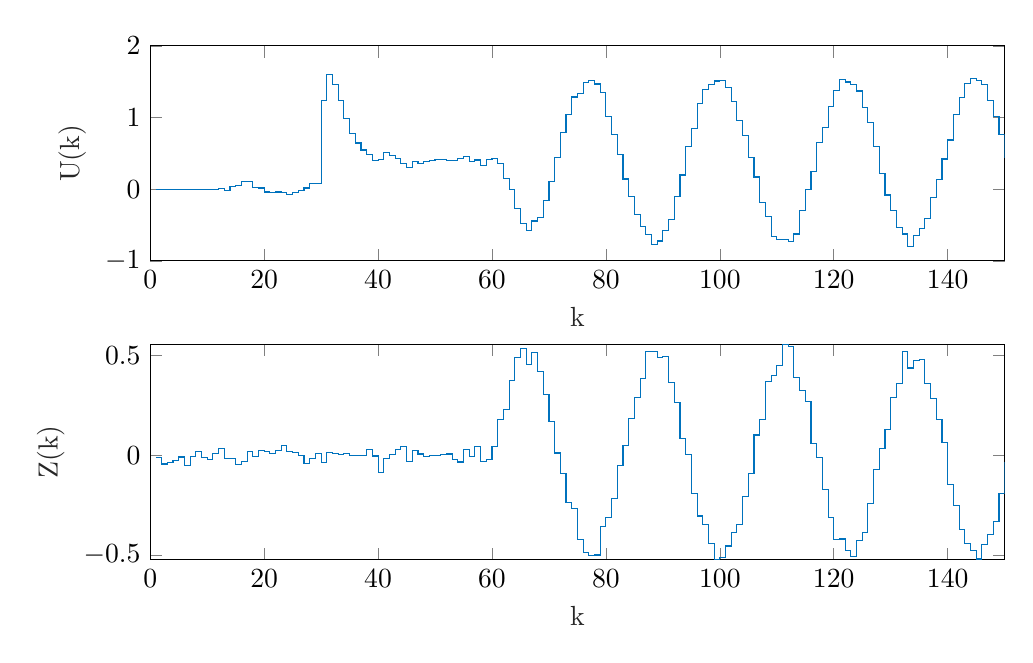
\begin{tikzpicture}

\begin{axis}[%
width=4.272in,
height=1.075in,
at={(0.717in,1.839in)},
scale only axis,
xmin=0,
xmax=150,
xlabel style={font=\color{white!15!black}},
xlabel={k},
ymin=-1,
ymax=2,
ylabel style={font=\color{white!15!black}},
ylabel={U(k)},
axis background/.style={fill=white}
]
\addplot[const plot, color=mycolor1, forget plot] table[row sep=crcr] {%
1	0\\
2	0\\
3	0\\
4	0\\
5	0\\
6	0\\
7	0\\
8	0\\
9	0\\
10	0\\
11	0\\
12	0.00736362754671591\\
13	-0.0160624325883666\\
14	0.0404043961983865\\
15	0.0549591080243713\\
16	0.109260568931026\\
17	0.100853982351326\\
18	0.0253072294760826\\
19	0.015321021791237\\
20	-0.0400803097390891\\
21	-0.0482448109032252\\
22	-0.0398254236240949\\
23	-0.0462963815948263\\
24	-0.0739029482253168\\
25	-0.0413273707423866\\
26	-0.0223355735545961\\
27	0.0157530128350385\\
28	0.0818714169883389\\
29	0.072926109735794\\
30	1.23883031546048\\
31	1.60397239568955\\
32	1.46558799300815\\
33	1.23604379508342\\
34	0.991731295418022\\
35	0.782178656233809\\
36	0.643699030789394\\
37	0.54620810536267\\
38	0.483754958610594\\
39	0.404575445933957\\
40	0.411368879671991\\
41	0.515170112776115\\
42	0.466076221805596\\
43	0.427757276036346\\
44	0.355992657441825\\
45	0.306805804352034\\
46	0.39056964707961\\
47	0.354951394799636\\
48	0.385871484814013\\
49	0.405217264696846\\
50	0.407706211608612\\
51	0.413210489262927\\
52	0.404282009974102\\
53	0.395682485967972\\
54	0.429701607049728\\
55	0.457080663009863\\
56	0.384315727997654\\
57	0.40657297323802\\
58	0.329487163658426\\
59	0.4140135920628\\
60	0.423426789294152\\
61	0.35847152081368\\
62	0.144098121029789\\
63	-0.00884547564501501\\
64	-0.264975926272828\\
65	-0.474390983025054\\
66	-0.573242522856034\\
67	-0.443828630035694\\
68	-0.399175072406509\\
69	-0.16146390089326\\
70	0.112617832903949\\
71	0.443013866359424\\
72	0.792773350825318\\
73	1.04570204698166\\
74	1.28650014437329\\
75	1.33859564754644\\
76	1.48425612224512\\
77	1.51749893247877\\
78	1.46659614476398\\
79	1.34876142988268\\
80	1.01894311843574\\
81	0.767706926636894\\
82	0.477993640330601\\
83	0.141788731344672\\
84	-0.107670325207461\\
85	-0.351590934938685\\
86	-0.517536999453197\\
87	-0.631147217614242\\
88	-0.766062432094818\\
89	-0.722968183286035\\
90	-0.579328167290488\\
91	-0.428399671152597\\
92	-0.105349901793887\\
93	0.197280955692214\\
94	0.600425796376072\\
95	0.850956850653366\\
96	1.19047410746618\\
97	1.39227003721158\\
98	1.45755594118747\\
99	1.50887132359919\\
100	1.52206594363862\\
101	1.41756927648137\\
102	1.21708993624895\\
103	0.961766004060622\\
104	0.747649846815367\\
105	0.443307316722845\\
106	0.170176989141394\\
107	-0.186278535622269\\
108	-0.382663142790877\\
109	-0.659605029322408\\
110	-0.706260592488187\\
111	-0.706992244223328\\
112	-0.733621563539725\\
113	-0.626021854641011\\
114	-0.300660767501889\\
115	-0.00736184472051388\\
116	0.249028179127083\\
117	0.646141317057361\\
118	0.863782206593481\\
119	1.14912951455021\\
120	1.37296955031968\\
121	1.52993693667958\\
122	1.4943389512448\\
123	1.45718334439727\\
124	1.37012963083526\\
125	1.1448380507425\\
126	0.9353160775521\\
127	0.597841788266556\\
128	0.214696744806207\\
129	-0.0814218816790386\\
130	-0.298612758188831\\
131	-0.529530367132049\\
132	-0.625260953691092\\
133	-0.796790729892282\\
134	-0.64167334421189\\
135	-0.550791979740045\\
136	-0.406708334077891\\
137	-0.120044361237163\\
138	0.137324630232317\\
139	0.420650983690489\\
140	0.686391147783828\\
141	1.0454813526345\\
142	1.27586559743302\\
143	1.47133032574543\\
144	1.54441221814875\\
145	1.51799917345082\\
146	1.46036517029778\\
147	1.24123531599499\\
148	1.01316256035993\\
149	0.76394230803024\\
150	0.441177836701096\\
};
\end{axis}

\begin{axis}[%
width=4.272in,
height=1.075in,
at={(0.717in,0.346in)},
scale only axis,
xmin=0,
xmax=150,
xlabel style={font=\color{white!15!black}},
xlabel={k},
ymin=-0.521017855307123,
ymax=0.556404933143915,
ylabel style={font=\color{white!15!black}},
ylabel={Z(k)},
axis background/.style={fill=white}
]
\addplot[const plot, color=mycolor1, forget plot] table[row sep=crcr] {%
1	-0.00821345639507819\\
2	-0.0428421881969322\\
3	-0.0366015298115334\\
4	-0.024096124429006\\
5	-0.00791516792870989\\
6	-0.0521384667174699\\
7	-0.00575504863351627\\
8	0.0194697397219508\\
9	-0.0119114863192416\\
10	-0.0220738133902148\\
11	0.00961719566440613\\
12	0.0348192043017277\\
13	-0.0141229840966605\\
14	-0.0147587371800649\\
15	-0.0454046355889962\\
16	-0.0309180980805826\\
17	0.0191600695646258\\
18	-0.00359407164580768\\
19	0.0241775591251869\\
20	0.0211840175792573\\
21	0.0118833236407034\\
22	0.0242436906736496\\
23	0.048176409800976\\
24	0.0182407826190953\\
25	0.0134704495271324\\
26	-0.00135759649092143\\
27	-0.0392838056850159\\
28	-0.015967973901705\\
29	0.0103043232072752\\
30	-0.0351462930236096\\
31	0.0148052882897143\\
32	0.0102019149126247\\
33	0.00316295557727557\\
34	0.00953219840932371\\
35	0.000753369569096519\\
36	-0.000697431932500447\\
37	-0.000276950024419697\\
38	0.0293919519736422\\
39	-0.00285972080105493\\
40	-0.0835203632103234\\
41	-0.0153734126014004\\
42	0.00619710357954776\\
43	0.0303490809595354\\
44	0.0436496894980746\\
45	-0.0297716943016982\\
46	0.0240607620886922\\
47	0.00752370517330569\\
48	-0.00658934735762414\\
49	0.000782322170900923\\
50	-0.000888318693824446\\
51	0.00443854535571105\\
52	0.00751313477833919\\
53	-0.0212362353253655\\
54	-0.0330458021302289\\
55	0.0305402227651014\\
56	-0.00694931135743456\\
57	0.0447315514229789\\
58	-0.0292253481586334\\
59	-0.0187883824178735\\
60	0.0449446760906472\\
61	0.181622106760085\\
62	0.231167831872316\\
63	0.376618916757131\\
64	0.490505763739525\\
65	0.533894406213104\\
66	0.45707204069725\\
67	0.516678503675773\\
68	0.418533041580582\\
69	0.306425397807076\\
70	0.170787652112084\\
71	0.0124181006999414\\
72	-0.0922792528457918\\
73	-0.234347046964146\\
74	-0.266776208840582\\
75	-0.421366087487956\\
76	-0.487642074229287\\
77	-0.500419457371631\\
78	-0.498838624138249\\
79	-0.356674117362049\\
80	-0.31240628714901\\
81	-0.215047765706894\\
82	-0.0500923123428492\\
83	0.0517058274264049\\
84	0.183984561433969\\
85	0.2894536706192\\
86	0.384031067431999\\
87	0.519740416079992\\
88	0.522850904905192\\
89	0.492625414854033\\
90	0.497543622352004\\
91	0.364152661376455\\
92	0.26447479853034\\
93	0.0827262786007183\\
94	0.00519686153422911\\
95	-0.192307073544353\\
96	-0.303262712888671\\
97	-0.34660640869076\\
98	-0.44126516489549\\
99	-0.521017855307123\\
100	-0.509256407831634\\
101	-0.453712689526292\\
102	-0.384613607379762\\
103	-0.345421378162904\\
104	-0.206826892351429\\
105	-0.0892254009792449\\
106	0.102625584159464\\
107	0.180526859057515\\
108	0.369171200607572\\
109	0.40060144204747\\
110	0.449680212650729\\
111	0.556404933143915\\
112	0.544960871418072\\
113	0.390932949304279\\
114	0.323972309179303\\
115	0.270595336454232\\
116	0.0588244639483252\\
117	-0.00820871267489531\\
118	-0.170233267715982\\
119	-0.313000523147682\\
120	-0.420390430166868\\
121	-0.418775541147117\\
122	-0.476715706108705\\
123	-0.5078227553448\\
124	-0.426607324668593\\
125	-0.38434519242426\\
126	-0.242089177109922\\
127	-0.0696536236517038\\
128	0.0364799160609692\\
129	0.131888550709027\\
130	0.291212440456367\\
131	0.360956300897808\\
132	0.520328965329816\\
133	0.438204973066564\\
134	0.474581513774828\\
135	0.482359727127619\\
136	0.35943991107949\\
137	0.283818688856025\\
138	0.180107107751742\\
139	0.0631155038422491\\
140	-0.143828226449222\\
141	-0.248959259718153\\
142	-0.368903954391837\\
143	-0.440863107043008\\
144	-0.475306792333295\\
145	-0.51895812545223\\
146	-0.448212240211377\\
147	-0.397836843788076\\
148	-0.332547740572066\\
149	-0.190816271464969\\
150	-0.0350518813672616\\
};
\end{axis}
\end{tikzpicture}%
\caption{Zakłócenie i sygnał sterujący- szum średni}
\end{figure}

\begin{figure}[H]
\centering
% This file was created by matlab2tikz.
%
%The latest updates can be retrieved from
%  http://www.mathworks.com/matlabcentral/fileexchange/22022-matlab2tikz-matlab2tikz
%where you can also make suggestions and rate matlab2tikz.
%
\definecolor{mycolor1}{rgb}{0.00000,0.44700,0.74100}%
\definecolor{mycolor2}{rgb}{0.85000,0.32500,0.09800}%
%
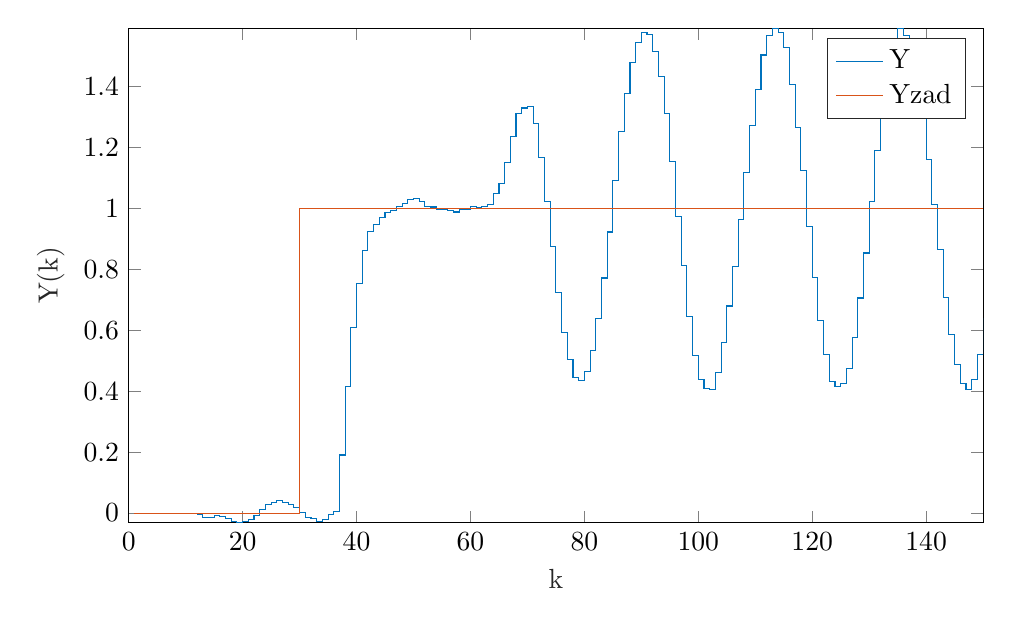
\begin{tikzpicture}

\begin{axis}[%
width=4.272in,
height=2.472in,
at={(0.717in,0.441in)},
scale only axis,
xmin=0,
xmax=150,
xlabel style={font=\color{white!15!black}},
xlabel={k},
ymin=-0.0313379684250232,
ymax=1.59173510806796,
ylabel style={font=\color{white!15!black}},
ylabel={Y(k)},
axis background/.style={fill=white},
legend style={legend cell align=left, align=left, draw=white!15!black}
]
\addplot[const plot, color=mycolor1] table[row sep=crcr] {%
1	0\\
2	0\\
3	0\\
4	0\\
5	0\\
6	0\\
7	0\\
8	0\\
9	0\\
10	0\\
11	0\\
12	-0.00610697189516439\\
13	-0.0133625443838905\\
14	-0.0131954648057447\\
15	-0.00776192647403886\\
16	-0.0126431581802659\\
17	-0.0169333344588578\\
18	-0.0267715488272743\\
19	-0.0313379684250232\\
20	-0.0285384359401706\\
21	-0.0222943357248857\\
22	-0.00854055827755179\\
23	0.0116301172573173\\
24	0.0273440233538207\\
25	0.033427586483142\\
26	0.0423542757030205\\
27	0.0361181764791491\\
28	0.0280512646191601\\
29	0.0187369231716221\\
30	0.00153681383638179\\
31	-0.0134494904829362\\
32	-0.0171694233929866\\
33	-0.0270982316316649\\
34	-0.0202778522273564\\
35	-0.00516040081805009\\
36	0.00623608422662193\\
37	0.19066179825924\\
38	0.416325291473013\\
39	0.607903689414484\\
40	0.754322707018864\\
41	0.861970381610019\\
42	0.925450927575138\\
43	0.948487545177236\\
44	0.970452425344302\\
45	0.986345067399863\\
46	0.99432986826537\\
47	1.00515305964797\\
48	1.01537262430309\\
49	1.02896241639698\\
50	1.03248299886268\\
51	1.02228028424092\\
52	1.00700295129217\\
53	1.00469474055983\\
54	0.998363428485713\\
55	0.997571358999585\\
56	0.993820229498338\\
57	0.988529272248833\\
58	0.997564850589736\\
59	0.996804149620801\\
60	1.00533289110514\\
61	1.00295994795789\\
62	1.00724506090503\\
63	1.01359934275883\\
64	1.04998218382462\\
65	1.08091377797073\\
66	1.1496737593946\\
67	1.23522872936044\\
68	1.31052022973486\\
69	1.32979838393785\\
70	1.33433430027157\\
71	1.27757324567918\\
72	1.16865694718949\\
73	1.02368497417707\\
74	0.875464357322714\\
75	0.724078937188886\\
76	0.591546280842658\\
77	0.505415331046481\\
78	0.446422515573049\\
79	0.434827689739059\\
80	0.46439810307279\\
81	0.53330531044027\\
82	0.639119447584405\\
83	0.771678865456005\\
84	0.922742323993681\\
85	1.09118412421368\\
86	1.2514908528901\\
87	1.37800788855228\\
88	1.47777443336862\\
89	1.54373619414653\\
90	1.57878201556712\\
91	1.56985668619985\\
92	1.51424694223384\\
93	1.43423661377559\\
94	1.31148169991747\\
95	1.15402201300669\\
96	0.974937002739612\\
97	0.81344644644403\\
98	0.646022649673574\\
99	0.517837994359871\\
100	0.437953151835934\\
101	0.407941990241035\\
102	0.405787192314739\\
103	0.461763982855803\\
104	0.560174742101307\\
105	0.679936936058839\\
106	0.810537581290622\\
107	0.965086163529416\\
108	1.11883942264606\\
109	1.27138363210191\\
110	1.38973969213241\\
111	1.50391424883981\\
112	1.56743598840642\\
113	1.59173510806796\\
114	1.57849070911962\\
115	1.52913675466952\\
116	1.40583811866535\\
117	1.26680609756248\\
118	1.12351853456431\\
119	0.941150916850047\\
120	0.773471683772734\\
121	0.633172417919594\\
122	0.519285813613129\\
123	0.433066335160665\\
124	0.41633066722255\\
125	0.425778380992544\\
126	0.475384465618684\\
127	0.576160823621116\\
128	0.705932547526483\\
129	0.853892987335142\\
130	1.02303753322325\\
131	1.18942222099247\\
132	1.32961009276209\\
133	1.45963153979494\\
134	1.54170624286637\\
135	1.58977539179643\\
136	1.56875218081519\\
137	1.51987670418738\\
138	1.43708680433343\\
139	1.31637030280166\\
140	1.16006738748106\\
141	1.01396074983543\\
142	0.86649415326897\\
143	0.708677400821659\\
144	0.584835512018856\\
145	0.486369318375361\\
146	0.426122000658813\\
147	0.407016345085725\\
148	0.438342817723465\\
149	0.521097566154491\\
150	0.641645806565739\\
};
\addlegendentry{Y}

\addplot[const plot, color=mycolor2] table[row sep=crcr] {%
1	0\\
2	0\\
3	0\\
4	0\\
5	0\\
6	0\\
7	0\\
8	0\\
9	0\\
10	0\\
11	0\\
12	0\\
13	0\\
14	0\\
15	0\\
16	0\\
17	0\\
18	0\\
19	0\\
20	0\\
21	0\\
22	0\\
23	0\\
24	0\\
25	0\\
26	0\\
27	0\\
28	0\\
29	0\\
30	1\\
31	1\\
32	1\\
33	1\\
34	1\\
35	1\\
36	1\\
37	1\\
38	1\\
39	1\\
40	1\\
41	1\\
42	1\\
43	1\\
44	1\\
45	1\\
46	1\\
47	1\\
48	1\\
49	1\\
50	1\\
51	1\\
52	1\\
53	1\\
54	1\\
55	1\\
56	1\\
57	1\\
58	1\\
59	1\\
60	1\\
61	1\\
62	1\\
63	1\\
64	1\\
65	1\\
66	1\\
67	1\\
68	1\\
69	1\\
70	1\\
71	1\\
72	1\\
73	1\\
74	1\\
75	1\\
76	1\\
77	1\\
78	1\\
79	1\\
80	1\\
81	1\\
82	1\\
83	1\\
84	1\\
85	1\\
86	1\\
87	1\\
88	1\\
89	1\\
90	1\\
91	1\\
92	1\\
93	1\\
94	1\\
95	1\\
96	1\\
97	1\\
98	1\\
99	1\\
100	1\\
101	1\\
102	1\\
103	1\\
104	1\\
105	1\\
106	1\\
107	1\\
108	1\\
109	1\\
110	1\\
111	1\\
112	1\\
113	1\\
114	1\\
115	1\\
116	1\\
117	1\\
118	1\\
119	1\\
120	1\\
121	1\\
122	1\\
123	1\\
124	1\\
125	1\\
126	1\\
127	1\\
128	1\\
129	1\\
130	1\\
131	1\\
132	1\\
133	1\\
134	1\\
135	1\\
136	1\\
137	1\\
138	1\\
139	1\\
140	1\\
141	1\\
142	1\\
143	1\\
144	1\\
145	1\\
146	1\\
147	1\\
148	1\\
149	1\\
150	1\\
};
\addlegendentry{Yzad}

\end{axis}
\end{tikzpicture}%
\caption{Wyjście dla pomiaru z szumem średnim (błąd $E=22,5508$)}
\end{figure}

\begin{figure}[H]
\centering
% This file was created by matlab2tikz.
%
%The latest updates can be retrieved from
%  http://www.mathworks.com/matlabcentral/fileexchange/22022-matlab2tikz-matlab2tikz
%where you can also make suggestions and rate matlab2tikz.
%
\definecolor{mycolor1}{rgb}{0.00000,0.44700,0.74100}%
%
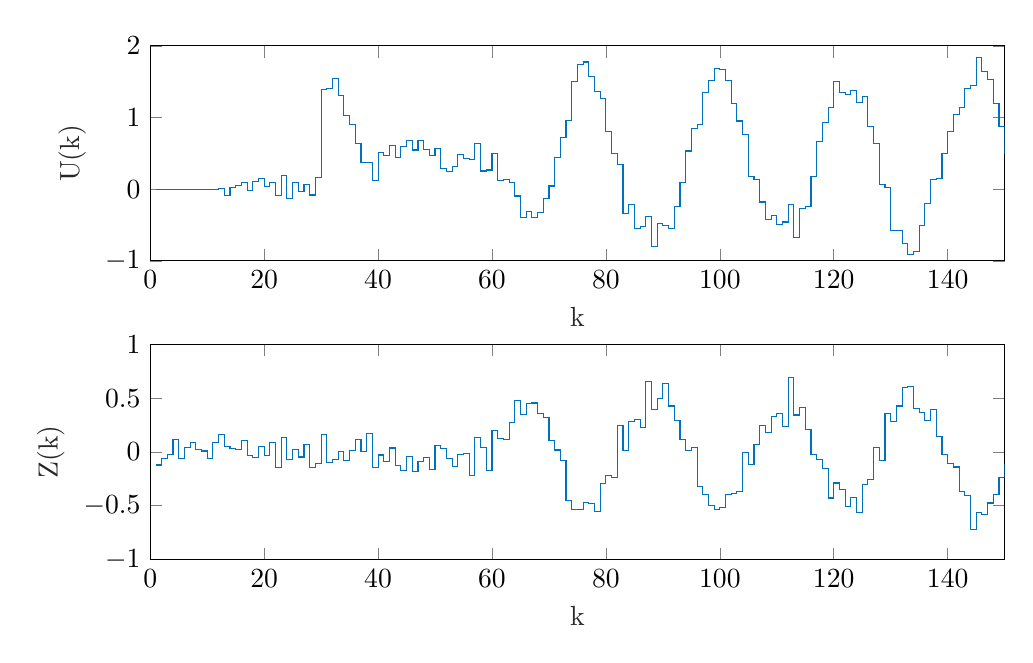
\begin{tikzpicture}

\begin{axis}[%
width=4.272in,
height=1.075in,
at={(0.717in,1.839in)},
scale only axis,
xmin=0,
xmax=150,
xlabel style={font=\color{white!15!black}},
xlabel={k},
ymin=-1,
ymax=2,
ylabel style={font=\color{white!15!black}},
ylabel={U(k)},
axis background/.style={fill=white}
]
\addplot[const plot, color=mycolor1, forget plot] table[row sep=crcr] {%
1	0\\
2	0\\
3	0\\
4	0\\
5	0\\
6	0\\
7	0\\
8	0\\
9	0\\
10	0\\
11	0\\
12	0.00324368789232185\\
13	-0.0832186160608578\\
14	0.0234590446708595\\
15	0.0554324983454778\\
16	0.0906861067889487\\
17	-0.0213083822744724\\
18	0.106163502367857\\
19	0.147634824270168\\
20	0.0381869235112201\\
21	0.0953510015872512\\
22	-0.0835174493495838\\
23	0.185316380993027\\
24	-0.125175706368705\\
25	0.0883554516046265\\
26	-0.0323516464756629\\
27	0.0687938238100707\\
28	-0.0809514579431054\\
29	0.168227410936538\\
30	1.38962504325928\\
31	1.39970319554812\\
32	1.53973126296579\\
33	1.30369829628368\\
34	1.02325407972807\\
35	0.908184424344121\\
36	0.637427156179882\\
37	0.366128547172871\\
38	0.370376016681494\\
39	0.126427289825198\\
40	0.50890999532876\\
41	0.46786679386732\\
42	0.604046072921393\\
43	0.437206138875684\\
44	0.593075171389021\\
45	0.677853131460056\\
46	0.546105181408531\\
47	0.676719792142314\\
48	0.548823134579967\\
49	0.471907639350824\\
50	0.56392350544659\\
51	0.285048558211537\\
52	0.24523412527991\\
53	0.320329412689597\\
54	0.484880448674022\\
55	0.42892009799224\\
56	0.407829572342065\\
57	0.642510064558163\\
58	0.252608357582889\\
59	0.267225272383404\\
60	0.49751340295468\\
61	0.117078838277651\\
62	0.138878886101115\\
63	0.0868815855763187\\
64	-0.094919212182722\\
65	-0.389736897360707\\
66	-0.310880634445116\\
67	-0.392476434792676\\
68	-0.325860155795656\\
69	-0.127051290165661\\
70	0.044059376817385\\
71	0.44658603894924\\
72	0.719935471358573\\
73	0.957922733495194\\
74	1.49880048543865\\
75	1.73404530047423\\
76	1.77481017946485\\
77	1.56953210645736\\
78	1.35958000781249\\
79	1.26118666791061\\
80	0.798528978559958\\
81	0.502295231172377\\
82	0.348810936321043\\
83	-0.343906099476875\\
84	-0.219161471631099\\
85	-0.551917023676755\\
86	-0.527014041048137\\
87	-0.375758644016504\\
88	-0.795488712024809\\
89	-0.47985092493841\\
90	-0.505479969327501\\
91	-0.549819042462364\\
92	-0.239593849081199\\
93	0.0874172223289448\\
94	0.532479384081418\\
95	0.844947389137553\\
96	0.902990267312811\\
97	1.34941088450374\\
98	1.51906160108137\\
99	1.68086973673354\\
100	1.66782129851089\\
101	1.51783240546951\\
102	1.19201541742265\\
103	0.950794993831345\\
104	0.762447737946286\\
105	0.177461847960062\\
106	0.129928585033505\\
107	-0.179069137144045\\
108	-0.418583329198181\\
109	-0.373700709523821\\
110	-0.498560778147848\\
111	-0.458929634624885\\
112	-0.21993337184856\\
113	-0.674223583469616\\
114	-0.27411153998649\\
115	-0.246734745755761\\
116	0.178156844410317\\
117	0.661411957305089\\
118	0.927899716492082\\
119	1.13570598954763\\
120	1.49801298190921\\
121	1.35269601983521\\
122	1.3255971678798\\
123	1.38193893471208\\
124	1.21405715543073\\
125	1.28803620667721\\
126	0.86866737490331\\
127	0.637741599810967\\
128	0.060864054108107\\
129	0.0276625408989819\\
130	-0.575687587801954\\
131	-0.574514061677072\\
132	-0.754560816466395\\
133	-0.906686818870102\\
134	-0.872680982720572\\
135	-0.501476886918432\\
136	-0.19547867652258\\
137	0.129101103413968\\
138	0.145409658017746\\
139	0.491413422889821\\
140	0.800720871837492\\
141	1.04195024135594\\
142	1.1346096195571\\
143	1.40067655852227\\
144	1.45004382692768\\
145	1.83093845713989\\
146	1.64593954380315\\
147	1.53392856852834\\
148	1.192777214245\\
149	0.877142577937881\\
150	0.488166702960397\\
};
\end{axis}

\begin{axis}[%
width=4.272in,
height=1.075in,
at={(0.717in,0.346in)},
scale only axis,
xmin=0,
xmax=150,
xlabel style={font=\color{white!15!black}},
xlabel={k},
ymin=-1,
ymax=1,
ylabel style={font=\color{white!15!black}},
ylabel={Z(k)},
axis background/.style={fill=white}
]
\addplot[const plot, color=mycolor1, forget plot] table[row sep=crcr] {%
1	-0.121417529661296\\
2	-0.0606400402810642\\
3	-0.0273702157088698\\
4	0.117574314851635\\
5	-0.0594572028552305\\
6	0.0372033911049199\\
7	0.0905823580174678\\
8	0.0231662966956191\\
9	0.0084797972206992\\
10	-0.061054743367174\\
11	0.0841319599238164\\
12	0.162861729235296\\
13	0.0475538005392531\\
14	0.0307314205467728\\
15	0.0235369783552629\\
16	0.103403848881578\\
17	-0.0330897452682976\\
18	-0.0512192994488433\\
19	0.0531863818361121\\
20	-0.030648126656273\\
21	0.0891823691199314\\
22	-0.146386882738798\\
23	0.13263660386309\\
24	-0.0730619104668757\\
25	0.0238549415338402\\
26	-0.046787928599774\\
27	0.0713570614848185\\
28	-0.141749625288212\\
29	-0.106729373133174\\
30	0.163237969705383\\
31	-0.0975389008770207\\
32	-0.0698361575607913\\
33	0.00623171020060246\\
34	-0.0798704973000339\\
35	0.0146706668329981\\
36	0.117592606433444\\
37	0.00686839767411369\\
38	0.172618638117959\\
39	-0.144974016310585\\
40	-0.0284642940549723\\
41	-0.0874041553991488\\
42	0.0368500196188389\\
43	-0.126166848520152\\
44	-0.175959450516116\\
45	-0.0393533130365602\\
46	-0.181503754424699\\
47	-0.0898105103831431\\
48	-0.0547302197513294\\
49	-0.167039209868734\\
50	0.056391937485226\\
51	0.0305612360273877\\
52	-0.0627148707686647\\
53	-0.139233918383177\\
54	-0.0275295627881658\\
55	-0.0167850126274036\\
56	-0.217294717941297\\
57	0.130741754247125\\
58	0.04355296971779\\
59	-0.175354588812438\\
60	0.197807947328765\\
61	0.121754987971753\\
62	0.116368620826331\\
63	0.277483959150128\\
64	0.474366820911612\\
65	0.34777074542478\\
66	0.450349534139364\\
67	0.455350379625331\\
68	0.355113095284557\\
69	0.319602758377346\\
70	0.10671964988907\\
71	0.0179138712569102\\
72	-0.0762112446470521\\
73	-0.448237146507341\\
74	-0.531649681693246\\
75	-0.534084142515634\\
76	-0.474173174909664\\
77	-0.479696359912881\\
78	-0.552574290935876\\
79	-0.290946832965375\\
80	-0.219250328909321\\
81	-0.235126766014637\\
82	0.246940442708463\\
83	0.016222426634184\\
84	0.285414868534048\\
85	0.300753379987339\\
86	0.231009668909553\\
87	0.656983425981\\
88	0.392193792434199\\
89	0.497249450025052\\
90	0.635728545074285\\
91	0.42767840834596\\
92	0.292402506884106\\
93	0.113085450549022\\
94	0.0146875818797266\\
95	0.0424779720417796\\
96	-0.318106559282738\\
97	-0.398782328820436\\
98	-0.497929657518012\\
99	-0.534638832394489\\
100	-0.51391468100712\\
101	-0.399934491290318\\
102	-0.382750476386639\\
103	-0.367372890731005\\
104	-0.00350141736477\\
105	-0.120117919513325\\
106	0.0718743089561674\\
107	0.242963030005894\\
108	0.178755249078182\\
109	0.331488961790831\\
110	0.355302315093584\\
111	0.233352761053212\\
112	0.6898802812288\\
113	0.343805436164683\\
114	0.40914986784909\\
115	0.210239107887603\\
116	-0.0235046463679003\\
117	-0.0665599315824533\\
118	-0.155683424778113\\
119	-0.429037602326312\\
120	-0.289413181836716\\
121	-0.352633750338359\\
122	-0.508938742015331\\
123	-0.426378262200406\\
124	-0.560886529252951\\
125	-0.299394230793753\\
126	-0.259630247239521\\
127	0.0427559329067452\\
128	-0.0760459004112\\
129	0.357062255767803\\
130	0.282216703070868\\
131	0.42757353697973\\
132	0.601425555645584\\
133	0.605221767029687\\
134	0.407850617010756\\
135	0.366440287794889\\
136	0.293899172666902\\
137	0.39072804451053\\
138	0.14583907783331\\
139	-0.0211275106994021\\
140	-0.106259680735257\\
141	-0.140010442111225\\
142	-0.369877328249327\\
143	-0.406322508705426\\
144	-0.718531488052545\\
145	-0.566154179241892\\
146	-0.58017262195686\\
147	-0.475245760611751\\
148	-0.393808096228376\\
149	-0.241753210889353\\
150	-0.115308686109502\\
};
\end{axis}
\end{tikzpicture}%
\caption{Zakłócenie i sygnał sterujący- szum duży}
\end{figure}

\begin{figure}[H]
\centering
% This file was created by matlab2tikz.
%
%The latest updates can be retrieved from
%  http://www.mathworks.com/matlabcentral/fileexchange/22022-matlab2tikz-matlab2tikz
%where you can also make suggestions and rate matlab2tikz.
%
\definecolor{mycolor1}{rgb}{0.00000,0.44700,0.74100}%
\definecolor{mycolor2}{rgb}{0.85000,0.32500,0.09800}%
%
\begin{tikzpicture}

\begin{axis}[%
width=4.272in,
height=3.472in,
at={(0.717in,0.441in)},
scale only axis,
xmin=0,
xmax=150,
xlabel style={font=\color{white!15!black}},
xlabel={k},
ymin=-0.0188652048941365,
ymax=2,
ylabel style={font=\color{white!15!black}},
ylabel={Y(k)},
axis background/.style={fill=white},
legend style={legend cell align=left, align=left, draw=white!15!black}
]
\addplot[const plot, color=mycolor1] table[row sep=crcr] {%
1	0\\
2	0\\
3	0\\
4	0\\
5	0\\
6	0\\
7	0\\
8	0\\
9	0\\
10	0\\
11	0\\
12	-0.00269012937841067\\
13	-0.0188652048941365\\
14	-0.00364896949049241\\
15	0.0259950216949079\\
16	0.0292339883474295\\
17	0.028914739931801\\
18	0.0273696239361059\\
19	0.0427927064421145\\
20	0.0163192719849326\\
21	0.00443575333291835\\
22	0.0200779316044247\\
23	0.0228418013820127\\
24	0.0337830747466491\\
25	0.0146701811668533\\
26	0.0611216132013507\\
27	0.0458076128020086\\
28	0.0605049708813649\\
29	0.0335231816795162\\
30	0.0724418405869809\\
31	0.0194266451040148\\
32	0.00989772187753173\\
33	0.0387519067714376\\
34	0.0262838931977876\\
35	-0.000876927418755225\\
36	0.026481103733563\\
37	0.215247075506651\\
38	0.414171450541569\\
39	0.642464825973987\\
40	0.798550790244159\\
41	0.93733443406347\\
42	0.984882207799394\\
43	1.01487906850937\\
44	0.991393099730144\\
45	0.99594321736274\\
46	0.930697771142147\\
47	0.917104547941327\\
48	0.927519867669372\\
49	0.928763853988976\\
50	0.925330348132385\\
51	0.952625912636967\\
52	0.968122964089486\\
53	1.00953299703183\\
54	1.06123807155597\\
55	1.07120249318332\\
56	1.05392467143132\\
57	1.07482369435565\\
58	1.05508912519212\\
59	0.989723129286152\\
60	1.01143170386858\\
61	1.03643432782836\\
62	1.00649098420924\\
63	1.05207536711386\\
64	1.11162345165898\\
65	1.10733608908083\\
66	1.13668273217508\\
67	1.23521406071321\\
68	1.24138700764157\\
69	1.26833269426577\\
70	1.28341125425861\\
71	1.24721910103792\\
72	1.16059305225085\\
73	1.04652883762254\\
74	0.910408145320121\\
75	0.775198069039614\\
76	0.605035223664573\\
77	0.459871853098285\\
78	0.388977564395576\\
79	0.380729093576964\\
80	0.411662832373514\\
81	0.510184448847906\\
82	0.694985722006711\\
83	0.890522765296725\\
84	1.04118328450198\\
85	1.24966688827712\\
86	1.37983884343122\\
87	1.48647042349522\\
88	1.54159936538084\\
89	1.55253437705247\\
90	1.54350705407061\\
91	1.49280264418731\\
92	1.41359092816365\\
93	1.36647299004057\\
94	1.29722183950333\\
95	1.14023209178952\\
96	1.00227179805944\\
97	0.85009763904081\\
98	0.708187979818548\\
99	0.549365415317837\\
100	0.437339631245194\\
101	0.383332638576244\\
102	0.377349490556697\\
103	0.390241509087679\\
104	0.496296748423716\\
105	0.627745985763463\\
106	0.781026581169674\\
107	0.998935606611188\\
108	1.15618928846502\\
109	1.29419665173674\\
110	1.42038699512824\\
111	1.49419495498133\\
112	1.50503934142805\\
113	1.50877554345088\\
114	1.43793339465472\\
115	1.42582637221255\\
116	1.34425520986939\\
117	1.25982895470856\\
118	1.14322898192475\\
119	1.02125695073277\\
120	0.83278041258066\\
121	0.699000474808178\\
122	0.525029970634317\\
123	0.458049222719562\\
124	0.457246607064673\\
125	0.468125858867085\\
126	0.53082101509477\\
127	0.619807924637339\\
128	0.739499161262456\\
129	0.857442804872731\\
130	1.03856219069873\\
131	1.15754631557984\\
132	1.36689911439647\\
133	1.48117001372397\\
134	1.57976436711296\\
135	1.61711243799991\\
136	1.64160745739361\\
137	1.52974521766093\\
138	1.41327046035357\\
139	1.26015437373077\\
140	1.11194304241634\\
141	0.92593868651241\\
142	0.772849126926958\\
143	0.659322264645004\\
144	0.596782194479661\\
145	0.497019662520364\\
146	0.452184520493078\\
147	0.397693863302896\\
148	0.420689648765706\\
149	0.458490167522489\\
150	0.559447505419244\\
};
\addlegendentry{Y}

\addplot[const plot, color=mycolor2] table[row sep=crcr] {%
1	0\\
2	0\\
3	0\\
4	0\\
5	0\\
6	0\\
7	0\\
8	0\\
9	0\\
10	0\\
11	0\\
12	0\\
13	0\\
14	0\\
15	0\\
16	0\\
17	0\\
18	0\\
19	0\\
20	0\\
21	0\\
22	0\\
23	0\\
24	0\\
25	0\\
26	0\\
27	0\\
28	0\\
29	0\\
30	1\\
31	1\\
32	1\\
33	1\\
34	1\\
35	1\\
36	1\\
37	1\\
38	1\\
39	1\\
40	1\\
41	1\\
42	1\\
43	1\\
44	1\\
45	1\\
46	1\\
47	1\\
48	1\\
49	1\\
50	1\\
51	1\\
52	1\\
53	1\\
54	1\\
55	1\\
56	1\\
57	1\\
58	1\\
59	1\\
60	1\\
61	1\\
62	1\\
63	1\\
64	1\\
65	1\\
66	1\\
67	1\\
68	1\\
69	1\\
70	1\\
71	1\\
72	1\\
73	1\\
74	1\\
75	1\\
76	1\\
77	1\\
78	1\\
79	1\\
80	1\\
81	1\\
82	1\\
83	1\\
84	1\\
85	1\\
86	1\\
87	1\\
88	1\\
89	1\\
90	1\\
91	1\\
92	1\\
93	1\\
94	1\\
95	1\\
96	1\\
97	1\\
98	1\\
99	1\\
100	1\\
101	1\\
102	1\\
103	1\\
104	1\\
105	1\\
106	1\\
107	1\\
108	1\\
109	1\\
110	1\\
111	1\\
112	1\\
113	1\\
114	1\\
115	1\\
116	1\\
117	1\\
118	1\\
119	1\\
120	1\\
121	1\\
122	1\\
123	1\\
124	1\\
125	1\\
126	1\\
127	1\\
128	1\\
129	1\\
130	1\\
131	1\\
132	1\\
133	1\\
134	1\\
135	1\\
136	1\\
137	1\\
138	1\\
139	1\\
140	1\\
141	1\\
142	1\\
143	1\\
144	1\\
145	1\\
146	1\\
147	1\\
148	1\\
149	1\\
150	1\\
};
\addlegendentry{Yzad}

\end{axis}
\end{tikzpicture}%
\caption{Wyjście dla pomiaru z szumem dużym (błąd $E=21,8056$)}
\end{figure}

\section{Wnioski}
Występowanie szumu pomiarowego pogarsza jakość regulacji.
Szum jest generowany w sposób losowy, dlatego też zwiększanie wartości błędów szumu pomiarowego, nie zawsze będzie skutkowało pogorszeniem regulacji. Widać to na przykładnie zakłócenia sinusoidalnego: nałożenie dużego szumu skutkowało mniejszym błędem niż w przypadku małego i średniego szumu.
\smallskip

